\documentclass{report}
\setlength{\parskip}{\baselineskip}%
\usepackage{amsmath}
\usepackage{amsfonts,stmaryrd,amssymb} % Math packages

\usepackage{enumerate} % Custom item numbers for enumerations
\usepackage{fontawesome}
\usepackage{setspace}
\usepackage{hyperref}
\usepackage{enumitem}
\usepackage{multicol}
\usepackage{xhfill}
\usepackage[p,osf]{cochineal}
\usepackage[scale=.95,type1]{cabin}
\usepackage[cochineal,bigdelims,cmintegrals,vvarbb]{newtxmath}
\usepackage[zerostyle=c,scaled=.94]{newtxtt}
\usepackage[cal=boondoxo]{mathalfa}
\usepackage[export]{adjustbox}
\usepackage{vwcol}  
\usepackage{fancyhdr}
\DeclareSymbolFont{yhlargesymbols}{OMX}{yhex}{m}{n}
\DeclareMathAccent{\wideparen}{\mathord}{yhlargesymbols}{"F3}

\hypersetup{
	colorlinks=false,
	linkcolor=black,
	filecolor=black,      
	urlcolor=black,
	pdftitle={Overleaf Example},
	pdfpagemode=FullScreen,
	urlbordercolor=white,
}

\urlstyle{same}


	
\newenvironment{cequation}{
	\makeatletter
	\setbool{@fleqn}{false}
	\makeatother
	\begin{equation*}
		}{\end{equation*}}
		
\newcommand{\sol}{\noindent\textbf{Solution:} }
%----------------------------------------------------------------------------------------

\newcommand{\exercise}[1]{%
	\subsection*{\faPencil\ \ Exercise #1\hspace{0.5em}\xrfill[0.175\baselineskip]{1pt}}
}

\newcommand{\practice}[1]{%
	\subsection*{\faFlag\ \ Practice #1\hspace{0.5em}\xrfill[0.175\baselineskip]{1pt}}
}

\newcommand{\revision}[1]{%
	\section*{\faGears\ \ Revision Exercise #1\hspace{0.5em}\xrfill[0.175\baselineskip]{1pt}}
}

\usepackage[ruled]{algorithm2e} % Algorithms

\usepackage[framemethod=tikz]{mdframed} % Allows defining custom boxed/framed environments

\usepackage{listings} % File listings, with syntax highlighting
\lstset{
	basicstyle=\ttfamily, % Typeset listings in monospace font
}

%----------------------------------------------------------------------------------------
%	DOCUMENT MARGINS
%----------------------------------------------------------------------------------------

\usepackage{geometry} % Required for adjusting page dimensions and margins

\geometry{
	paper=a4paper, % Paper size, change to letterpaper for US letter size
	top=2.5cm, % Top margin
	bottom=3cm, % Bottom margin
	left=2.5cm, % Left margin
	right=2.5cm, % Right margin
	headheight=14pt, % Header height
	footskip=1.5cm, % Space from the bottom margin to the baseline of the footer
	headsep=1.2cm, % Space from the top margin to the baseline of the header
	%showframe, % Uncomment to show how the type block is set on the page
}

%----------------------------------------------------------------------------------------
%	FONTS
%----------------------------------------------------------------------------------------

\usepackage[utf8]{inputenc} % Required for inputting international characters
\usepackage[T1]{fontenc} % Output font encoding for international characters

%----------------------------------------------------------------------------------------
%	COMMAND LINE ENVIRONMENT
%----------------------------------------------------------------------------------------

% Usage:
% \begin{commandline}
%	\begin{verbatim}
%		$ ls
%		
%		Applications	Desktop	...
%	\end{verbatim}
% \end{commandline}

\mdfdefinestyle{commandline}{
	leftmargin=10pt,
	rightmargin=10pt,
	innerleftmargin=15pt,
	middlelinecolor=black!50!white,
	middlelinewidth=2pt,
	frametitlerule=false,
	backgroundcolor=black!5!white,
	frametitle={Command Line},
	frametitlefont={\normalfont\sffamily\color{white}\hspace{-1em}},
	frametitlebackgroundcolor=black!50!white,
	nobreak,
}

% Define a custom environment for command-line snapshots
\newenvironment{commandline}{
	\medskip
	\begin{mdframed}[style=commandline]
		}{
	\end{mdframed}
	\medskip
}

%----------------------------------------------------------------------------------------
%	FILE CONTENTS ENVIRONMENT
%----------------------------------------------------------------------------------------

% Usage:
% \begin{file}[optional filename, defaults to "File"]
%	File contents, for example, with a listings environment
% \end{file}

\mdfdefinestyle{file}{
	innertopmargin=1.6\baselineskip,
	innerbottommargin=0.8\baselineskip,
	topline=false, bottomline=false,
	leftline=false, rightline=false,
	leftmargin=2cm,
	rightmargin=2cm,
	singleextra={%
		\draw[fill=black!10!white](P)++(0,-1.2em)rectangle(P-|O);
		\node[anchor=north west]
		at(P-|O){\ttfamily\mdfilename};
		%
		\def\l{3em}
		\draw(O-|P)++(-\l,0)--++(\l,\l)--(P)--(P-|O)--(O)--cycle;
		\draw(O-|P)++(-\l,0)--++(0,\l)--++(\l,0);
	},
	nobreak,
}

% Define a custom environment for file contents
\newenvironment{file}[1][File]{ % Set the default filename to "File"
	\medskip
	\newcommand{\mdfilename}{#1}
	\begin{mdframed}[style=file]
		}{
	\end{mdframed}
	\medskip
}

%----------------------------------------------------------------------------------------
%	NUMBERED QUESTIONS ENVIRONMENT
%----------------------------------------------------------------------------------------

% Usage:
% \begin{question}[optional title]
%	Question contents
% \end{question}

\mdfdefinestyle{question}{
	innertopmargin=1.2\baselineskip,
	innerbottommargin=0.8\baselineskip,
	roundcorner=5pt,
	nobreak,
	singleextra={%
		\draw(P-|O)node[xshift=1em,anchor=west,fill=white,draw,rounded corners=3pt]{%
			\faCaretRight\ \textbf{Example \theQuestion\questionTitle}};
	},
}

\newcounter{Question} % Stores the current question number that gets iterated with each new question

% Define a custom environment for numbered questions
\newenvironment{question}[1][\unskip]{
	\bigskip
	\stepcounter{Question}
	\newcommand{\questionTitle}{~#1}
	\begin{mdframed}[style=question]
		}{
	\end{mdframed}
	\medskip
}

%----------------------------------------------------------------------------------------
%	SOLUTIONS ENVIRONMENT
%----------------------------------------------------------------------------------------

% Usage:
% \begin{solution}
%	Solution contents
% \end{solution}

\mdfdefinestyle{solution}{
	innertopmargin=1.2\baselineskip,
	innerbottommargin=0.8\baselineskip,
	roundcorner=5pt,
	nobreak,
	singleextra={%
		\draw(P-|O)node[xshift=1em,anchor=west,fill=white,draw,rounded corners=5pt]{解};
	},
}

% Define a custom environment for solutions
\newenvironment{solution}{
	\begin{mdframed}[style=solution]
		}{
	\end{mdframed}
}

%----------------------------------------------------------------------------------------
%	WARNING TEXT ENVIRONMENT
%----------------------------------------------------------------------------------------

% Usage:
% \begin{warn}[optional title, defaults to "Warning:"]
%	Contents
% \end{warn}

\mdfdefinestyle{warning}{
	topline=false, bottomline=false,
	leftline=false, rightline=false,
	nobreak,
	singleextra={%
		\draw(P-|O)++(-0.5em,0)node(tmp1){};
		\draw(P-|O)++(0.5em,0)node(tmp2){};
		\fill[black,rotate around={45:(P-|O)}](tmp1)rectangle(tmp2);
		\node at(P-|O){\color{white}\scriptsize\bf !};
		\draw[very thick](P-|O)++(0,-1em)--(O);%--(O-|P);
	}
}

% Define a custom environment for warning text
\newenvironment{warn}[1][Warning:]{ % Set the default warning to "Warning:"
	\medskip
	\begin{mdframed}[style=warning]
		\noindent{\textbf{#1}}
		}{
	\end{mdframed}
	\vspace{-0.5cm}
}

%----------------------------------------------------------------------------------------
%	INFORMATION ENVIRONMENT
%----------------------------------------------------------------------------------------

% Usage:
% \begin{info}[optional title, defaults to "Info:"]
% 	contents
% 	\end{info}

\mdfdefinestyle{info}{%
	topline=false, bottomline=false,
	leftline=false, rightline=false,
	nobreak,
	singleextra={%
		\fill[black](P-|O)circle[radius=0.6em];
		\node at(P-|O){\color{white}\scriptsize\bf \faInfo};
		\draw[very thick](P-|O)++(0,-0.8em)--(O);%--(O-|P);
	}
}

% Define a custom environment for information
\newenvironment{info}[1][Info:]{ % Set the default title to "Info:"
	\medskip
	\begin{mdframed}[style=info]
		\noindent{\textbf{#1}}
		}{
	\end{mdframed}
	\vspace{-0.5cm}
	
}

\mdfdefinestyle{explore}{%
	topline=false, bottomline=false,
	leftline=false, rightline=false,
	nobreak,
	singleextra={%
		\fill[black](P-|O)circle[radius=0.6em];
		\node at(P-|O){\color{white}\scriptsize\bf \faFlask};
		\draw[very thick](P-|O)++(0,-0.8em)--(O);%--(O-|P);
	}
}

% Define a custom environment for warning text
\newenvironment{explore}[1][Exploration Activity:]{ % Set the default warning to "Warning:"
	\medskip
	\begin{mdframed}[style=explore]
		\noindent{\large\textbf{#1}}
		}{
	\end{mdframed}
	\vspace{-0.5cm}
}

\mdfdefinestyle{think}{%
	topline=false, bottomline=false,
	leftline=false, rightline=false,
	nobreak,
	singleextra={%
		\fill[black](P-|O)circle[radius=0.6em];
		\node at(P-|O){\color{white}\scriptsize\bf \faQuestion};
		\draw[very thick](P-|O)++(0,-0.8em)--(O);%--(O-|P);
	}
}

% Define a custom environment for warning text
\newenvironment{think}[1][Think about It:]{ % Set the default warning to "Warning:"
	\medskip
	\begin{mdframed}[style=think]
		\noindent{\large\textbf{#1}}
		}{
	\end{mdframed}
	\vspace{-0.5cm}
}





\allowdisplaybreaks

\begin{document}
\pagestyle{fancy}
%... then configure it.
\fancyhead{} % clear all header fields
\fancyhead[RO,LE]{\thepage}
\fancyhead[LO,RE]{\leftmark}
\fancyfoot{} % clear all footer fields

\fancyfoot[LO,RE]{Dong Zong Addmath Textbook Senior 1 Volume II}
\fancyfoot[RO,RE]{\thepage}

\onehalfspacing
\setcounter{chapter}{9}

\chapter{Applications of Trigonometry}

\section{Law of Sine}

To find unknown sides and angles based on known sides and angles in a triangle is called solving a triangle. For any triangle (acute, right, or obtuse), the law of sine or the colaw of sine can be used, which describe the relationships between the sides and angles.

In triangle $\triangle ABC$, where the three internal angles $A$, $B$, and $C$ are represented by the lengths of their opposite sides as $a$, $b$, and $c$ respectively.

First, let's consider the acute triangle $\triangle ABC$ as shown in the figure below. Draw the altitude $CD$ to divide triangle $\triangle ABC$ into two right triangles: $\triangle ACD$ and $\triangle BCD$.

\vspace{-2em}
\begin{vwcol}[widths={0.7,0.3}, sep=8mm, rule=0pt]
    ~
    
    In triangle $\triangle ACD$, $\begin{aligned}[t]
        \sin A&=\dfrac{CD}{b} \\
        \therefore CD&=b \sin A\ \cdots\ (1)
        \end{aligned}$
        
        In triangle $\triangle BCD$, $\begin{aligned}[t]
        \sin B &= \dfrac{CD}{a} \\
        \therefore CD &= a \sin B\ \cdots\ (2)
        \end{aligned}$
        
        Comparing $(1)$ and $(2)$, we get $\begin{aligned}[t]
            b \sin A&=a \sin B
            \therefore \dfrac{a}{\sin A}&=\dfrac{b}{\sin B}
        \end{aligned}$
        
        Similarly, it can be proved that: $\dfrac{b}{\sin B}=\dfrac{c}{\sin C}$.
        \vspace{3em}
        
        \parbox{0.2\textwidth}{
            \vspace{4em}
            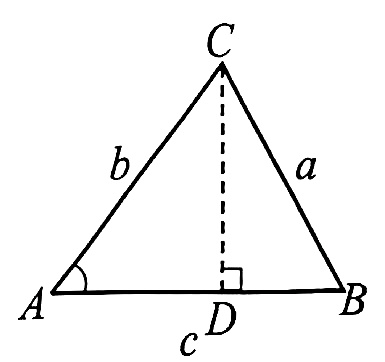
\includegraphics[width=0.2\textwidth]{assets/10-2.jpg}
        }
\end{vwcol}
\vspace{-6em}
These relationships also hold for obtuse and right triangles.

\begin{info}[Law of Sine]
    \begin{vwcol}[widths={0.7,0.3}, sep=8mm, rule=0pt]
        In any triangle, the ratio of the length of a side to the sine of its opposite angle is constant, namely:
        $$\dfrac{a}{\sin A}=\dfrac{b}{\sin B}=\dfrac{c}{\sin C}$$

        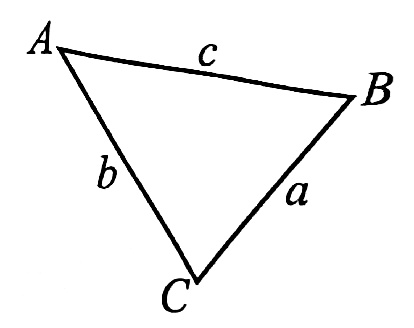
\includegraphics[width=0.2\textwidth]{assets/10-3.jpg}
    \end{vwcol}
\end{info}

Using the law of sine and the triangle angle sum theorem, we can solve problems involving the following two types of arbitrary triangles:
\begin{itemize}
    \item Given two angles and any one side, find the other two sides and one angle;
    \item Given two sides and one of their opposite angles, find the opposite angle of the other side, thus determining the other sides and angles.
\end{itemize}

\subsection*{Given Two Angles and Any One Side}

Generally, to solve a triangle given two angles and any one side, you can first use the triangle angle sum theorem to find the measure of the third angle. Then, you can use the law of sine to find the lengths of the remaining two sides.

\begin{question}
    In $\triangle DEF$, $D=60^\circ$, $E=72^\circ$, and $DE=7 \mathrm{~cm}$. Find the lengths of $DF$ and $EF$.

    \sol{}

    \begin{vwcol}[widths={0.6,0.4}, sep=8mm, rule=0pt,justify=flushleft]
        \noindent $F=180^{\circ}-60^{\circ}-72^{\circ}=48^{\circ}$

    \noindent Using the law of sine, we get $\dfrac{D F}{\sin 72^{\circ}}=\dfrac{7}{\sin 48^{\circ}}$

    \noindent $
    D F=\dfrac{7}{\sin 48^{\circ}} \times \sin 72^{\circ}=8.96 \mathrm{~cm}
    $

    \noindent $\begin{aligned}[t]
        \text{Using the law of sine again, we get }\dfrac{E F}{\sin 60^{\circ}}&=\dfrac{7}{\sin 48^{\circ}}\\
        E F=\dfrac{7}{\sin 48^{\circ}} \times \sin 60^{\circ}&=8.16 \mathrm{~cm}
    \end{aligned}$

    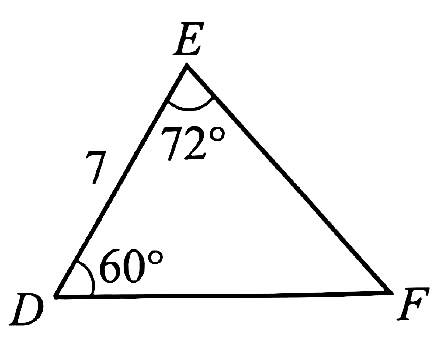
\includegraphics[width=0.2\textwidth]{assets/10-4.jpg}
    \end{vwcol}
\end{question}

\begin{question}
   \begin{multicols*}{2}
    As shown in the figure on the right, if a cable $AC$ of a bridge is $100 \mathrm{~m}$ long and makes an angle of $20^\circ$ with the bridge deck, and another cable $AB$ makes an angle of $40^\circ$ with the bridge deck, find the length of $AB$.
    \begin{center}
        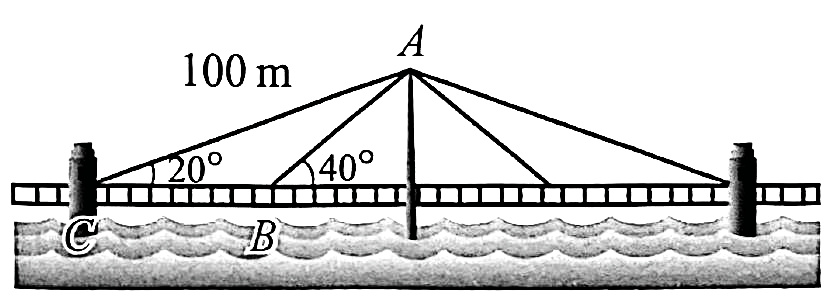
\includegraphics[width=0.4\textwidth]{assets/10-5.jpg}
    \end{center}
   \end{multicols*}

    \sol{}

    \noindent In $\triangle ABC$, $\angle CBA = 180^\circ - 40^\circ = 140^\circ$.

    \noindent $\begin{aligned}[t]
        \text{Using the law of sine, we get }\dfrac{AB}{\sin 20^\circ}&=\dfrac{100}{\sin 140^\circ}\\
        \therefore A B=\dfrac{100}{\sin 140^{\circ}} \times \sin 20^{\circ}&=53.21 \mathrm{~m} 
    \end{aligned}$
\end{question}

\newpage
\section*{Given Two Sides and One of Their Opposite Angles}

Generally, to solve a triangle given two sides and one of their opposite angles, you can first use the law of sine to find one angle. Then, you can use either the triangle angle sum theorem or the law of sine again to find the third angle, and finally, you can use the law of sine to find the remaining side.

\begin{question}
    In $\triangle ABC$, $A=30^\circ$, $BC=1 \mathrm{~cm}$, and $AC=\sqrt{3} \mathrm{~cm}$. Find the angle $B$ and the length of $AB$.

    \sol{}

    \begin{vwcol}[widths={0.6,0.4}, sep=8mm, rule=0pt,justify=flushleft]
        \noindent Using the law of sine, we get $\begin{aligned}[t]
            \dfrac{1}{\sin 30^{\circ}} &=\dfrac{\sqrt{3}}{\sin B} \\
            \sin B &=\dfrac{\sqrt{3}}{2} \\
            \therefore B &=60^{\circ} \text { or } 120^{\circ}
        \end{aligned}$
    
        \noindent When $\begin{aligned}[t] B=60^{\circ},\ C & =180^{\circ}-30^{\circ}-60^{\circ}=90^{\circ} \\ \dfrac{1}{\sin 30^{\circ}} & =\dfrac{A B}{\sin 90^{\circ}}\\ AB&=2 \mathrm{~cm} \end{aligned}$
    
        \noindent $\begin{gathered}\text { When } B=120^{\circ},\ C=180^{\circ}-30^{\circ}-120^{\circ}=30^{\circ} \\ \dfrac{1}{\sin 30^{\circ}}=\dfrac{A B}{\sin 30^{\circ}} \\ A B=1 \mathrm{~cm}\end{gathered}$

        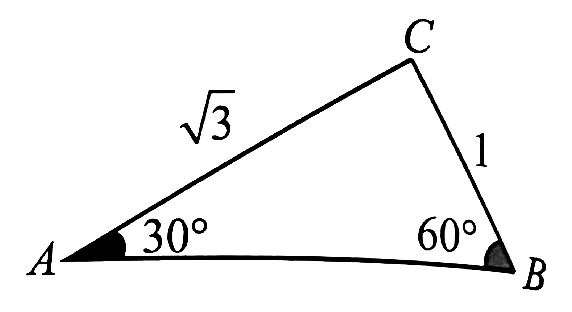
\includegraphics[width=0.25\textwidth]{assets/10-6.jpg}

        \vspace{3em}
        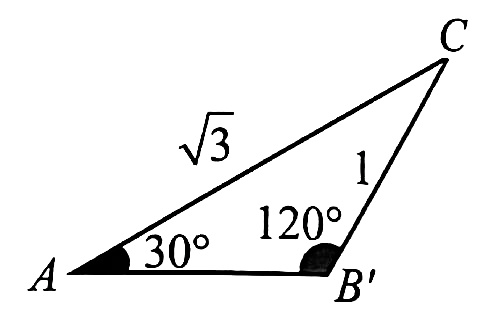
\includegraphics[width=0.25\textwidth]{assets/10-7.jpg}
    \end{vwcol}
\end{question}

\begin{vwcol}[widths={0.6,0.4}, sep=8mm, rule=0pt,justify=flushleft]
    From the example above, we can see that if the given conditions are two sides of a triangle and one of their opposite angles, using the law of sines to find an angle can result in two possible solutions: an acute angle and an obtuse angle. Therefore, it is impossible to uniquely determine the shape of the triangle.

    In shown in the figure to the right, after drawing $A=30^\circ$ and $AC=\sqrt{3}$ on the line $AP$, we draw an arc with $C$ as the center and radius of $1$. This arc intersects the line $AP$ at $B$ and $B'$. From this, we can see that both $\triangle ABC$ and $\triangle AB'C$ both satisfy the conditions of Example 3.

    \vspace{6em}

    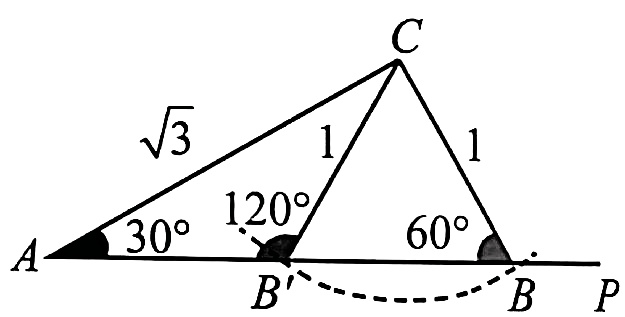
\includegraphics[width=0.3\textwidth]{assets/10-8.jpg}
\end{vwcol}

\newpage

\begin{question}
    In $\triangle ABC$, $a=60 \mathrm{~cm}$, $b=50 \mathrm{~cm}$, and $A=38^\circ$. Solve for $\triangle ABC$.

    \sol{}

    \begin{vwcol}[widths={0.6,0.4}, sep=8mm, rule=0pt,justify=flushleft]
        \noindent Using the law of sines, we get $\begin{aligned}[t]
            \dfrac{60}{\sin 38^{\circ}} & =\dfrac{50}{\sin B} \\ \sin B & =\dfrac{50}{60} \sin 38^{\circ} \\ \therefore B & =30.87^{\circ} \text { or } 149.13^{\circ}\end{aligned}$
    
            \vspace{1em}
            \noindent When $B=30.87^{\circ}, C=180^{\circ}-38^{\circ}-30.87^{\circ}=111.13^{\circ}$

        \vspace{3em}
        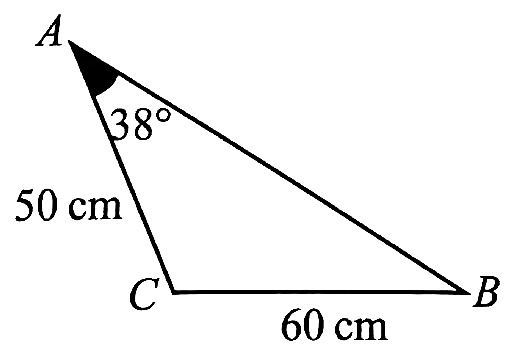
\includegraphics[width=0.25\textwidth]{assets/10-9.jpg}
    \end{vwcol}

    \vspace{-2em}
        \noindent Using the law of sines again, we get $\begin{aligned}[t] \dfrac{60}{\sin 38^{\circ}} & =\dfrac{c}{\sin 111.13^{\circ}} \\ c & =\dfrac{60}{\sin 38^{\circ}} \times \sin 111.13^{\circ} \\ & =90.90 \mathrm{~cm}\end{aligned}$

        \noindent When $B=149.13^{\circ}, A+B=38^{\circ}+149.13^{\circ}=187.13^{\circ}>180^{\circ}$ (rejected).

        \noindent Hence, $B=30.87^{\circ}, C=111.13^{\circ}, c=90.90 \mathrm{~cm}$.
\end{question}

\begin{question}
    In $\triangle ABC$, $a=10 \mathrm{~cm}$, $b=12 \mathrm{~cm}$, and $A=100^\circ$. Solve for $\triangle ABC$.

    \sol{}

    \noindent We can use the relationship "the larger side is opposite the larger angle" to deduce:

    \vspace{-1em}
\noindent \qquad    $
\because b>a, \quad \therefore B>A=100^\circ
$

\vspace{-1em}
\noindent Therefore, a contradiction arises: $A+B>200^\circ$.

\vspace{-1em}
\noindent From this, we can conclude that a triangle satisfying the given conditions does not exist.
\end{question}

\practice{10.1a}

Given the following conditions, solve for triangle $ABC$.
\vspace{-1em}
\begin{enumerate}
    \item $B C=8 \mathrm{~cm}, A=60^{\circ}, A C=6 \mathrm{~cm}$
    \item $A B=6 \mathrm{~km}, C=50^{\circ}, B C=8 \mathrm{~km}$
    \item $B C=5 \mathrm{~m}, B=100^{\circ}, A C=8 \mathrm{~m}$
\end{enumerate}

\subsection*{Radius of Circumscribed Circle of a Triangle}

Given any triangle $\triangle ABC$, consider its \textbf{circumcircle} with center $O$. There are three possible cases: the center $O$ lies on an edge of $\triangle ABC$, the center $O$ lies inside $\triangle ABC$, or the center $O$ lies outside $\triangle ABC$. We can derive the law of sines by considering the radius of the circumcircle of the triangle.

    \begin{enumerate}[label=(\arabic*)]
    \item \parbox[t][][t]{0.9\textwidth}{
        ~
        \vspace{-1.1em}
        \begin{vwcol}[widths={0.7,0.3}, sep=8mm, rule=0pt]
            As shown in the figure to the right, $\triangle ABC$ is a right triangle. Let the radius of the circumcircle be $R$. Then we have:
        \begin{flalign*}
            BC&=2R=a  &\\
        \sin A&=\sin 90^{\circ}=1 \\
        \text{Therefore } \dfrac{a}{\sin A}&=2R
        \end{flalign*}
    
        \parbox{0.2\textwidth}{
            \vspace{1em}
            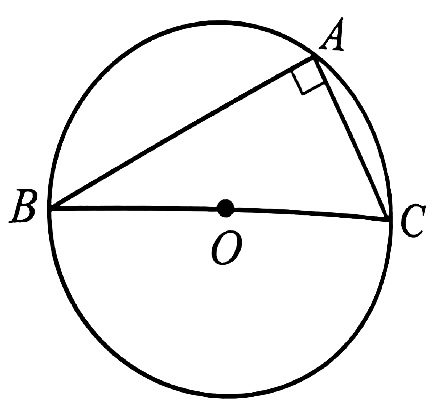
\includegraphics[width=0.2\textwidth]{assets/10-10.jpg}
        }
        \end{vwcol}
    }

    \vspace{-3em}
    \item \parbox[t][][t]{0.9\textwidth}{
        ~
        \vspace{-1.1em}
        \begin{vwcol}[widths={0.7,0.3}, sep=8mm, rule=0pt]
            As shown in the figure to the right, $\triangle ABC$ is an acute triangle. Let point $B$ be the diameter $BD$, and connect $CD$, then $\triangle BCD$ is a right triangle.

            \noindent From the central angle $\wideparen{BC}$, we have $A=D$.

            \noindent Therefore, $\sin D=\dfrac{a}{2R}=\sin A$.

            \noindent So, $\dfrac{a}{\sin A}=2R$.
    
            \parbox{0.2\textwidth}{
                \vspace{1em}
                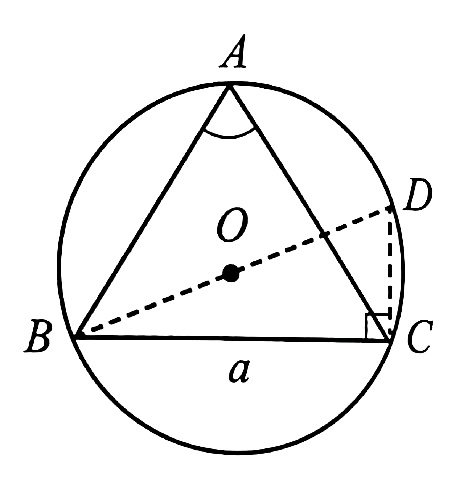
\includegraphics[width=0.2\textwidth]{assets/10-11.jpg}
            }
        \end{vwcol}
    }

    \vspace{-3em}
    \item \parbox[t][][t]{0.9\textwidth}{
        ~
        \vspace{-1.1em}
        \begin{vwcol}[widths={0.7,0.3}, sep=8mm, rule=0pt]
            As shown in the figure below, $\triangle ABC$ is an obtuse triangle. 
            
            \noindent Let point $B$ be the diameter $BD$, and connect $CD$, 
            
            \noindent then $\triangle BCD$ is a right triangle. 
            
            \noindent By the property of a cyclic quadrilateral, we have $A+D=180^\circ$. 
            
            \noindent Therefore, $\sin A=\sin (180^\circ-D)=\sin D=\dfrac{a}{2R}$.

            \noindent Hence $\dfrac{a}{\sin A}=2R$.
    
            \parbox{0.2\textwidth}{
                \vspace{1em}
                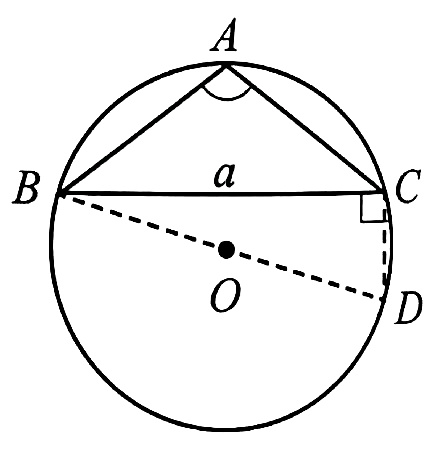
\includegraphics[width=0.2\textwidth]{assets/10-12.jpg}
            }
        \end{vwcol}
    }
    \end{enumerate}

    From the above three cases, we see that $\dfrac{a}{\sin A}=2R$ holds true. Since $A$ is any angle of $\triangle ABC$, the same holds for $B$ and $C$:
    
    \begin{info}[Radius of Circumscribed Circle]
        $$
            \dfrac{a}{\sin A}=\dfrac{b}{\sin B}=\dfrac{c}{\sin C}=2R
        $$
    \end{info}

    According to the basic properties of proportions, the above equations can also be written as:
    $$
    a: b: c=\sin A: \sin B: \sin C
    $$

    \vspace{-1em}
    This implies that the ratio of the lengths of the sides of a triangle is equal to the ratio of the sines of its angles.

    \begin{question}
        In $\triangle ABC$, $A: B: C=5: 7: 3$, and the perimeter of $\triangle ABC$ is $100 \mathrm{~cm}$. Find the length of the longest side of $\triangle ABC$ and its circumradius $R$.

        \sol{}
        
        \noindent $\begin{aligned} & A=\dfrac{5}{3+5+7} \times 180^{\circ}=60^{\circ} \\ & B=\dfrac{7}{3+5+7} \times 180^{\circ}=84^{\circ} \\ & C=\dfrac{3}{3+5+7} \times 180^{\circ}=36^{\circ}\end{aligned}$

        \noindent Since the largest angle is $B$, the longest side is its opposite side $b$. Using the properties of ratio,
        
        \noindent $\begin{aligned} \because a: b: c & =\sin A: \sin B: \sin C \\ \dfrac{b}{a+b+c} & =\dfrac{\sin B}{\sin A+\sin B+\sin C} \\ \therefore b & =\dfrac{\sin 84^{\circ}}{\sin 60^{\circ}+\sin 84^{\circ}+\sin 36^{\circ}} \times 100=40.62 \mathrm{~cm}\end{aligned}$

        \noindent Using the law of sines, we get $2R=\dfrac{40.62}{\sin 84^\circ}=40.84$, so the circumradius $R$ of triangle ABC is $20.42 \mathrm{~cm}$.
    \end{question}

    \practice{10.1b}
    \begin{vwcol}[widths={0.75,0.25}, sep=8mm, rule=0pt]
        \parbox{0.7\textwidth}{
            \begin{enumerate}
                \item In $\triangle ABC$, $A: B: C=2: 3: 5$, and the perimeter of $\triangle ABC$ is $80 \mathrm{~cm}$. Find the length of the shortest side.
        
                \item Find the radius of the circle shown in the right figure, as well as the lengths of $AB$ and $BC$.
            \end{enumerate}
        }

        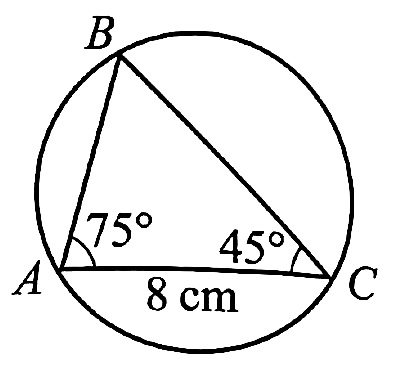
\includegraphics[width=0.2\textwidth]{assets/10-13.jpg}
    \end{vwcol}
    \vspace{-2em}

    \exercise{10.1}

    \begin{enumerate}
        \item \parbox[t]{0.9\textwidth}{
            ~
            \vspace{-1.1em}
            \begin{vwcol}[widths={0.7,0.3}, sep=8mm, rule=0pt]
                In the figure on the right, $\angle A = 77^\circ, \angle B = 56^\circ$, and $AC = 9 \mathrm{~cm}$.

                \noindent\parbox{0.5\textwidth}{
                    \begin{enumerate}
                        \item Find the lengths of $BC$ and $AB$.
            
                        \item Find the radius of the circumcircle of $\triangle ABC$.
                    \end{enumerate}
                }
    
                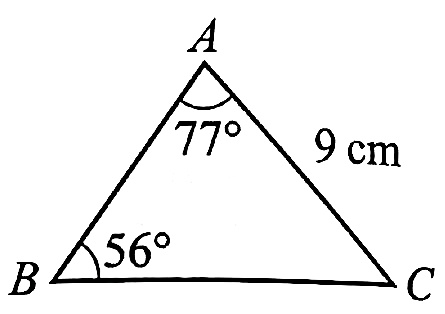
\includegraphics[width=0.2\textwidth]{assets/10-14.jpg}
            \end{vwcol}
        }

        \item \parbox[t]{0.9\textwidth}{
            ~
            \vspace{-1.1em}
            \begin{vwcol}[widths={0.7,0.3}, sep=8mm, rule=0pt]
                As shown in the figure on the right, two observation stations $A$ and $B$ on the ground simultaneously spot aircraft $C$. Angles $\angle BAC = 76^\circ$ and $\angle ABC = 74^\circ$ are measured at $A$ and $B$ respectively. Given that $A$ and $B$ are $5 \mathrm{~km}$ apart, find the distance between point $B$ and the aircraft.
    
                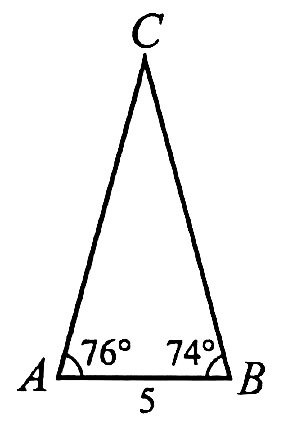
\includegraphics[width=0.14\textwidth]{assets/10-15.jpg}
            \end{vwcol}
        }

        \item \parbox[t]{0.9\textwidth}{
            ~
            \vspace{-1.1em}
            \begin{vwcol}[widths={0.7,0.3}, sep=8mm, rule=0pt]
                In the figure on the right, the circumradius of $\triangle ABC$ is $6 \mathrm{~cm}$, $AC = 9 \mathrm{~cm}$, and $BC = 10 \mathrm{~cm}$. Find the length of $AB$.
    
                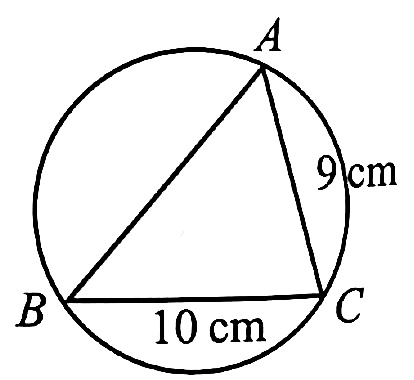
\includegraphics[width=0.2\textwidth]{assets/10-16.jpg}
            \end{vwcol}
        }

        \vspace{-2.5em}
        \item Based on the following conditions, sketch and solve $\triangle ABC$ (if possible).

        \begin{enumerate}
            \item $AB = 6 \mathrm{~m}, C = 40^\circ, BC = 10 \mathrm{~m}$
            
            \item $BC = 9 \mathrm{~cm}, B = 60^\circ, AC = 8 \mathrm{~cm}$
            
            \item $BC = 10 \mathrm{~km}, A = 40^\circ, AC = 7 \mathrm{~km}$
        \end{enumerate}

        \item If the perimeter of $\triangle PQR$ is $100 \mathrm{~cm}$ and $\angle P: \angle Q: \angle R = 1: 2: 6$, find the length of $PR$.

        \item In $\triangle ABC$, if $\angle A: \angle C = 3: 2$ and $\angle B: \angle C = 2: 3$, and the length of the shortest side is $5 \mathrm{~cm}$, find the perimeter of $\triangle ABC$.

        \item \parbox[t]{0.9\textwidth}{
            ~
            \vspace{-1.1em}
            \begin{vwcol}[widths={0.7,0.3}, sep=8mm, rule=0pt]
                In the figure on the right, $A$ is an acute angle, $ACD$ is a straight line, $AB = 9 \mathrm{~cm}$, $CD = 5 \mathrm{~cm}$, $\angle ACB = 48^\circ$, and $\angle CBD = 16^\circ$. Find:

                \noindent \parbox{0.5\textwidth}{
                    \begin{enumerate}
                        \item The length of $BC$.
                        \item The measure of angle $A$.
                        \item The length of $AD$.
                        \item With the given conditions, let $A'$ be a point on the line $AC$ such that $A'B = AB$. Draw $\triangle A'BC$.
                    \end{enumerate}}
    
                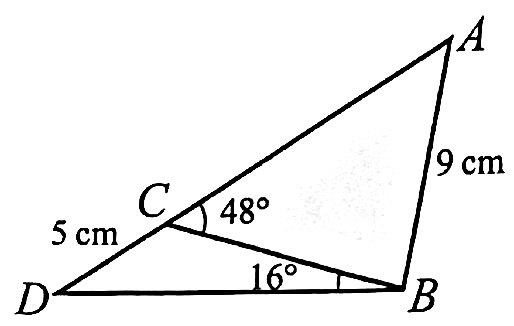
\includegraphics[width=0.25\textwidth]{assets/10-17.jpg}
            \end{vwcol}
        }
        
        \vspace{-2em}
        \item \parbox[t]{0.9\textwidth}{
            ~
            \vspace{-1.1em}
            \begin{vwcol}[widths={0.7,0.3}, sep=8mm, rule=0pt]
            In the figure on the right, find the lengths of $BD$ and $AB$.

            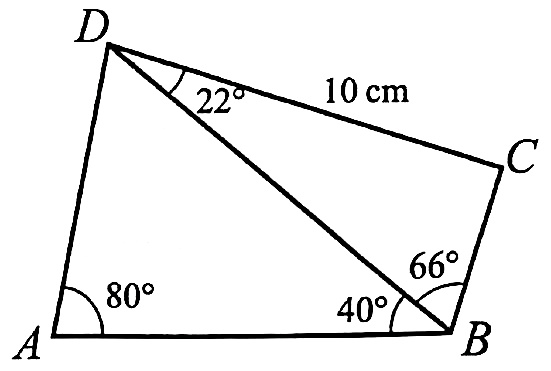
\includegraphics[width=0.23\textwidth]{assets/10-18.jpg}
            \end{vwcol}
        }
        
        \vspace{4em}
        \item \parbox[t]{0.9\textwidth}{
            ~
            \vspace{-1.1em}
            \begin{vwcol}[widths={0.7,0.3}, sep=8mm, rule=0pt]
            In the figure on the right, find the length of $CD$.

            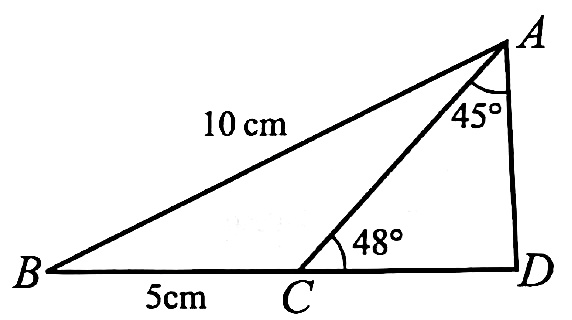
\includegraphics[width=0.25\textwidth]{assets/10-19.jpg}
            \end{vwcol}
        }
    \end{enumerate}

    \section{Law of Cosine}

    \vspace{-1em}
    \begin{vwcol}[widths={0.6,0.4}, sep=8mm, rule=0pt]
        In the right figure, $\triangle ABC$ is an acute triangle. Draw a perpendicular line from $C$ to $AB$.
    
        \noindent Let $CD = h$ and $AD = x$. Thus, $DB = c - x$. 

        \noindent In $\triangle ACD$, $h^2 = b^2 - x^2\ \cdots\ (1)$
        
        \noindent In $\triangle BCD$, $h^2 = a^2 - (c - x)^2\ \cdots\ (2)$

        \noindent Comparing (1) and (2), we get
        \vspace{-0.5em}
        $$\begin{aligned}[t]
            a^2 - (c - x)^2 &= b^2 - x^2 &&&&&&&&&& \\
                a^2 - c^2 + 2cx - x^2 &= b^2 - x^2 \\
                a^2 &= b^2 + c^2 - 2cx
        \end{aligned}$$

        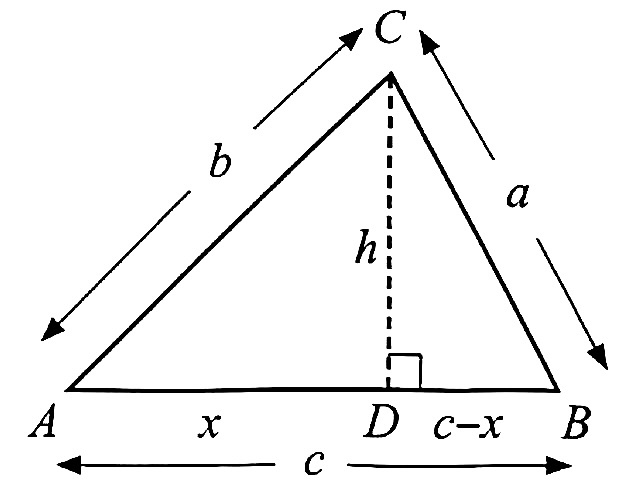
\includegraphics[width=0.3\textwidth]{assets/10-20.jpg}
    \end{vwcol}
    \vspace{-3em}

    \noindent In $\triangle ACD$, $\cos A = \dfrac{x}{b}$, hence $x = b \cos A$. Substituting into the above equation, we get
    $
    a^2 = b^2 + c^2 - 2cb \cos A
    $

    \vspace{-1em}
    \noindent Similarly, we can prove that $b^2 = c^2 + a^2 - 2ca \cos B$ and $c^2 = a^2 + b^2 - 2ab \cos C$. 
    
    \noindent These relations hold for any triangle.
    
    \newpage
    \begin{info}[Law of Cosine]
        \begin{vwcol}[widths={0.6,0.4}, sep=8mm, rule=0pt]
            Knowing any two sides of a triangle and their included angle, we can determine the third side.
            \begin{align*}
                a^2 &= b^2 + c^2 - 2bc \cos A \\
                b^2 &= c^2 + a^2 - 2ca \cos B \\
                c^2 &= a^2 + b^2 - 2ab \cos C
            \end{align*}
    
            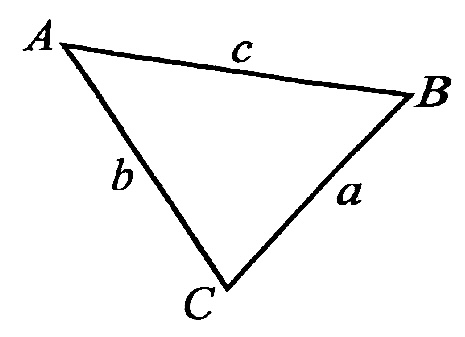
\includegraphics[width=0.25\textwidth]{assets/10-21.jpg}
        \end{vwcol}
    \end{info}

    Furthermore, the formula for the law of cosine can be written in the following form:
    $$
    \cos A=\dfrac{b^{2}+c^{2}-a^{2}}{2 b c}
    $$

    \vspace{-1em}
    From this, it can be seen that given the three sides of a triangle, the respective interior angles of the triangle can be determined using the cosine law.

    Using the cosine law, we can solve the following two types of problems for any triangle:
    \vspace{-1em}
    \begin{itemize}
        \item Given three sides, find the three angles.
        \item Given two sides and their included angle, find the third side and the other two angles.
    \end{itemize}

    \begin{think}

    \noindent When $\angle A=90^{\circ}$, which theorem will the cosine law become?
    \end{think}

    \subsection*{Given Three Sides}

    In general, given the three sides of a triangle, we can use the cosine law to determine each angles.

    \begin{question}
        Given that in $\triangle ABC$, $AB = 7 \mathrm{~cm}$, $BC = 10 \mathrm{~cm}$, and $AC = 12 \mathrm{~cm}$, find the three interior angles.

        \sol{}
        
        \begin{vwcol}[widths={0.6,0.4}, sep=8mm, rule=0pt,justify=flushleft]
            \noindent Using the law of cosine, we get $\begin{aligned}[t] \cos A&=\dfrac{12^2+7^2-10^2}{2 \times 12 \times 7}=\dfrac{31}{56} \\ \therefore A&=56.39^{\circ}\end{aligned}$

            \vspace{0.5em}
            \noindent Using the law of cosine, we get $\begin{aligned}[t] \cos B&=\dfrac{10^2+7^2-12^2}{2 \times 10 \times 7}=\dfrac{1}{28} \\ \therefore B&=87.95^{\circ}\end{aligned}$

            \vspace{0.5em}
            \noindent $\therefore$ In $\triangle A B C$, $C=180^{\circ}-56.39^{\circ}-87.95^{\circ}=35.66^{\circ}$
            \vspace{3em}

            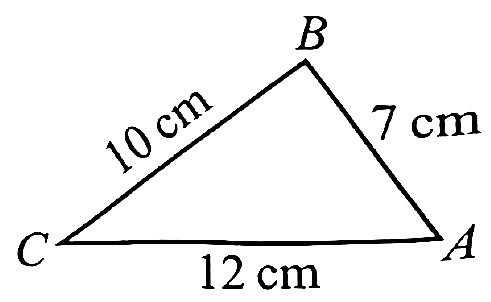
\includegraphics[width=0.25\textwidth]{assets/10-22.jpg}
        \end{vwcol}
        \vspace{-1em}
    \end{question}

    \begin{question}
        \begin{vwcol}[widths={0.6,0.4}, sep=8mm, rule=0pt]
            Xiao Ling found that Jupiter, Venus, and Mercury in the sky overlap exactly with the "V" made by her right hand. It is known that Xiao Ling's thumb is about $3$ cm long, her index finger is about $5$ cm long, and the distance between the tips of the two fingers is about $7$ cm. What is the approximate angle between Jupiter, Venus, and Mercury at the moment?

            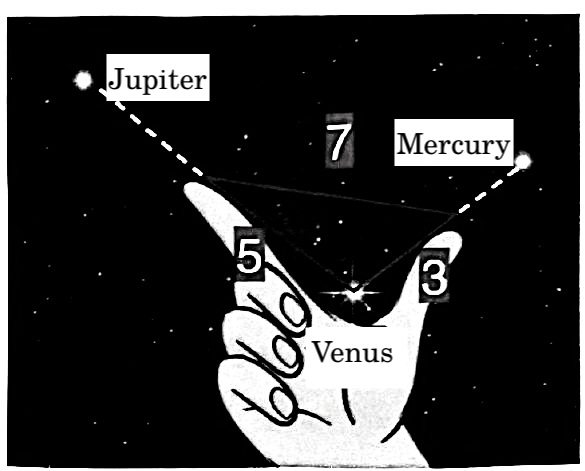
\includegraphics[width=0.3\textwidth]{assets/10-23.jpg}
        \end{vwcol}

        \sol{}

        \noindent Let $\theta$ be the angle between Xiao Ling's thumb and index finger.

        \noindent Using the cosine law, we have $\begin{aligned}[t] \cos \theta&=\dfrac{3^2+5^2-7^2}{2 \times 3 \times 5}=-\dfrac{1}{2} \\ \therefore \theta&=120^{\circ}\end{aligned}$

        \noindent Since the "V" made by Xiao Ling's right hand overlaps with Jupiter, Venus, and Mercury, the approximate angle between these planets is $120^\circ$.
    \end{question}

    \vspace{-2em}   
    \subsection*{Given Two Sides and Their Included Angle}
    
    Generally speaking, when given two sides and the angle between them, to solve the triangle, you can first use the law of cosine to find the third side, and then find the other two angles.

    \begin{question}
        Given that in $\triangle ABC$, $AB = 7$ cm, $BC = 5$ cm, and $\angle B = 75^\circ$, solve for $\triangle ABC$.

        \sol{}
        \begin{vwcol}[widths={0.6,0.4}, sep=8mm, rule=0pt,justify=flushleft]
            \noindent Using the law of cosine, we get $\begin{aligned}[t] A C^2 & =5^2+7^2-2 \times 5 \times 7 \times \cos 75^{\circ} \\ \therefore A C & =7.48 \mathrm{~cm}\end{aligned}$

            \vspace{0.5em}
            \noindent Using the law of cosine, we get $\begin{aligned}[t] \cos C&=\dfrac{5^2+A C^2-7^2}{2 \times 5 \times A C}=0.4265 \\ \therefore C&=64.75^{\circ}\end{aligned}$

            \vspace{0.5em}
            \noindent $\therefore$ In $\triangle A B C$, $A=180^{\circ}-75^{\circ}-64.75^{\circ}=40.25^{\circ}$

            \vspace{3em}    
            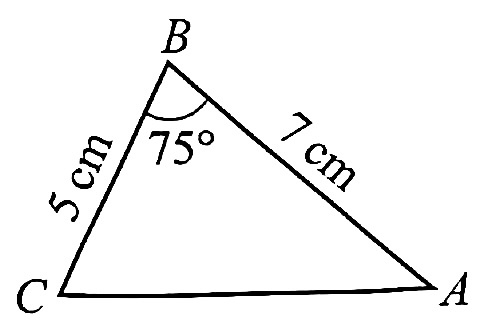
\includegraphics[width=0.25\textwidth]{assets/10-24.jpg}
        \end{vwcol}
        \vspace{-1em}
    \end{question}

    \vspace{-2em}
    \practice{10.2}
    \begin{enumerate}
        \item In $\triangle ABC$, if $AC = 4 \mathrm{~cm}$, $BC = 2\sqrt{7} \mathrm{~cm}$, and $\angle A = 60^\circ$, find the length of $AB$.

        \item In $\triangle DEF$, if the ratios of the sides are $DE : EF : FD = 6 : 8 : 5$, find the largest interior angle of $\triangle DEF$.

        \item In $\triangle ABC$, if $a^2 + b^2 - c^2 = \sqrt{2}ab$, find angle $C$.
    \end{enumerate}

    \exercise{10.2}
    \begin{enumerate}
        \item \parbox[t]{0.9\textwidth}{
            ~
            \vspace{-1.1em}
            \begin{vwcol}[widths={0.7,0.3}, sep=8mm, rule=0pt]
                In the figure on the right, the lengths of the sides of $\triangle ABC$ are $7 \mathrm{~cm}, 8 \mathrm{~cm}$, and $10 \mathrm{~cm}$. Find $\angle ACB$.
    
                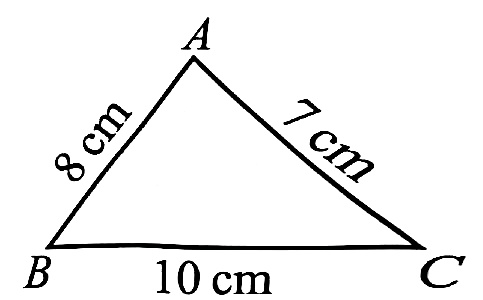
\includegraphics[width=0.23\textwidth]{assets/10-25.jpg}
            \end{vwcol}
        }

        \vspace{3em}
        \item \parbox[t]{0.9\textwidth}{
            ~
            \vspace{-1.1em}
            \begin{vwcol}[widths={0.7,0.3}, sep=8mm, rule=0pt]
                In $\triangle PQR$, $PR = 8 \mathrm{~cm}, QR = 9 \mathrm{~cm}$, and $R = 80^\circ$. Find:
                
                \noindent \parbox{0.3\textwidth}{
                    \begin{enumerate}
                        \item The length of $PQ$;
                        \item $\angle QPR$.
                    \end{enumerate}}
                \vfill\null
    
                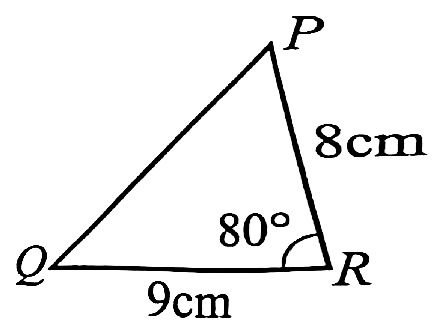
\includegraphics[width=0.2\textwidth]{assets/10-26.jpg}
            \end{vwcol}
        }

        \item \parbox[t]{0.9\textwidth}{
            ~
            \vspace{-1.1em}
            \begin{vwcol}[widths={0.6,0.4}, sep=8mm, rule=0pt]
                As shown in the figure on the right, a hill is located on the line segment connecting points $A$ and $B$. From an external point $C$ on the hill, it is measured that $AC = 800 \mathrm{~m}$, $BC = 600 \mathrm{~m}$, and $\angle ACB = 120^\circ$. Find the distance $AB$.
    
                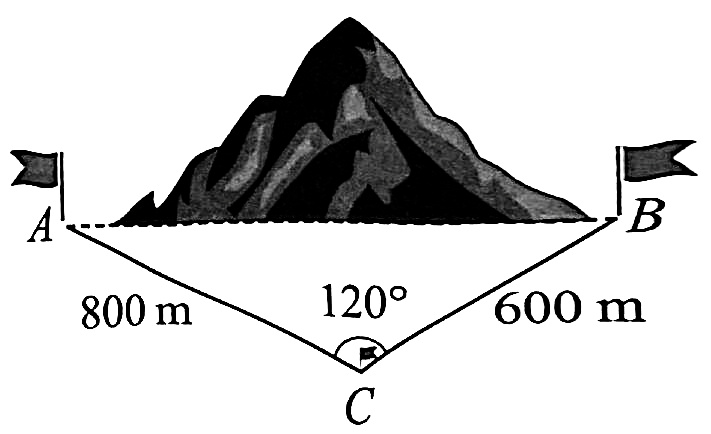
\includegraphics[width=0.3\textwidth]{assets/10-27.jpg}
            \end{vwcol}
        }

        \vspace{2em}
        \item \parbox[t]{0.9\textwidth}{
            ~
            \vspace{-1.1em}
            \begin{vwcol}[widths={0.6,0.4}, sep=8mm, rule=0pt]
                As shown in the figure on the right, $A$ and $B$ are located on opposite banks of a river, while $A$, $C$, and $D$ are three points on a straight highway. The distance between points $A$ and $C$ is 50 meters, and the distance between points $A$ and $D$ is 200 meters. Xiao Ming measured $\angle ACB = 60^\circ$ at point $C$ and $\angle ADB = 30^\circ$ at point $D$. Find the straight-line distance between $A$ and $B$.
    
                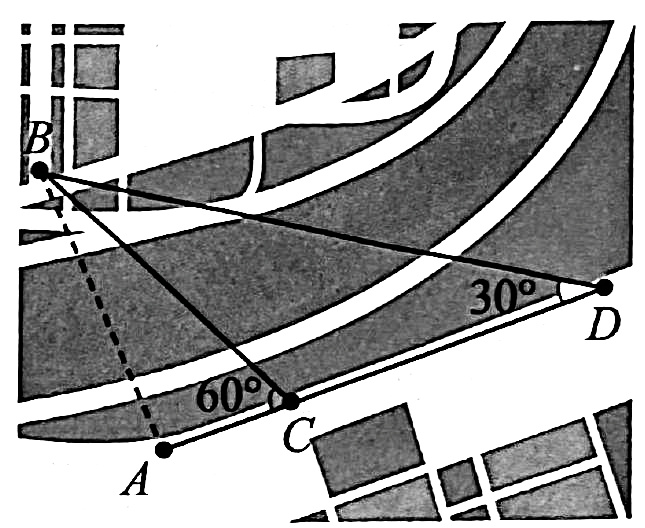
\includegraphics[width=0.3\textwidth]{assets/10-28.jpg}
            \end{vwcol}
        }

        \item Given that a wireless network base station is equidistant from three receiving stations $A$, $B$, and $C$, and $AB = 700 \mathrm{~m}$, $AC = 800 \mathrm{~m}$, and $BC = 900 \mathrm{~m}$. Find the distance between the base station and the receiving stations.

        \item If the lengths of the sides of a triangle are $m, n$, and $\sqrt{m^2 + mn + n^2}$, find the maximum interior angle.

        \item Given that $\triangle ABC$ is an obtuse triangle with side lengths $6, 8$, and $x$. Find the possible values of $x$.

        \item In $\triangle ABC$, if $\sin A: \sin B: \sin C = 6: 5: 4$. Find $\cos A: \cos B: \cos C$.

        \item \parbox[t]{0.9\textwidth}{
            ~
            \vspace{-1.1em}
            \begin{vwcol}[widths={0.7,0.3}, sep=8mm, rule=0pt]
                In quadrilateral $ABCD$, $\angle DCB = 105^\circ$, $\angle DAB = 48^\circ$, and $AB = 8 \mathrm{~cm}, AB = 8 \mathrm{~cm}$. Given that $BD$ is a diagonal and $\angle CBD = 33^\circ$. Find the length of $CD$.
    
                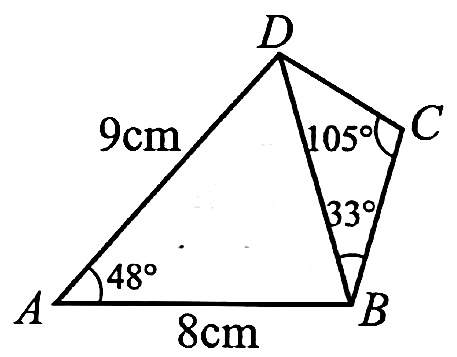
\includegraphics[width=0.23\textwidth]{assets/10-29.jpg}
            \end{vwcol}
        }

        \vspace{4em}
        \item \parbox[t]{0.9\textwidth}{
            ~
            \vspace{-1.3em}
            \begin{vwcol}[widths={0.7,0.3}, sep=8mm, rule=0pt]
                In the figure on the right, $PQRS$ is a parallelogram.

                \noindent If $PQ = 10 \mathrm{~cm}, PS = 8 \mathrm{~cm}$, and $\angle SPQ = 65^\circ$, find:

                \vspace{0.5em}
                \noindent\parbox{0.5\textwidth}{
                    \begin{enumerate}
                        \item The lengths of the two diagonals;
                        \item The acute angle between the two diagonals.
                    \end{enumerate}}
    
                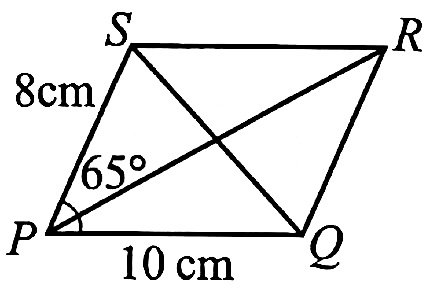
\includegraphics[width=0.23\textwidth]{assets/10-30.jpg}
            \end{vwcol}
        }

        \item \parbox[t]{0.9\textwidth}{
            ~
            \vspace{-1.1em}
            \begin{vwcol}[widths={0.7,0.3}, sep=8mm, rule=0pt]
                In the figure on the right, $ABCD$ is a parallelogram. Find the lengths of $AB$ and the other diagonal $BD$.
    
                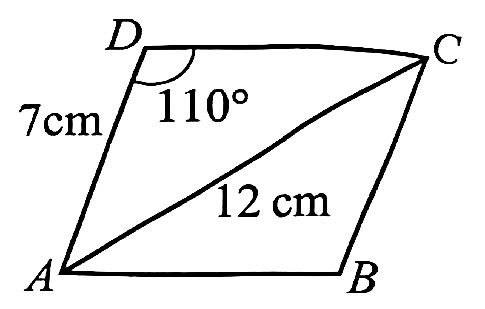
\includegraphics[width=0.25\textwidth]{assets/10-31.jpg}
            \end{vwcol}
        }

        \vspace{3em}
        \item \parbox[t]{0.9\textwidth}{
            ~
            \vspace{-1.1em}
            \begin{vwcol}[widths={0.7,0.3}, sep=8mm, rule=0pt]
                In the figure on the right, $AM$ is the median on side $BC$.

                \noindent If $AB = 6 \mathrm{~cm}$, $AC = 11 \mathrm{~cm}$, and $\angle BAC = 76^\circ$, find:
                
                \noindent\parbox{0.5\textwidth}{
                    \begin{enumerate}
                        \item the length of $BC$;
                        \item $\angle B$;
                        \item the length of $AM$;
                        \item $\angle BAM$.
                    \end{enumerate}}
    
                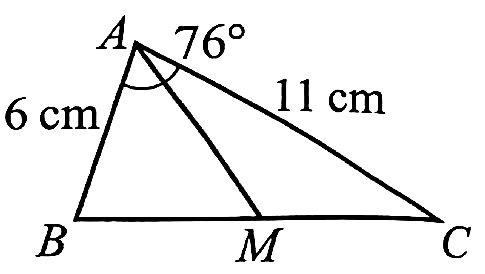
\includegraphics[width=0.25\textwidth]{assets/10-32.jpg}
            \end{vwcol}
        }

    \vspace{-3em}
    \item \parbox[t]{0.9\textwidth}{
        ~
        \vspace{-1.1em}
        \begin{vwcol}[widths={0.7,0.3}, sep=8mm, rule=0pt]
            In the figure on the right, $\angle BAC = 80^\circ$, $AD$ is the angle bisector of $\angle BAC$. If $AB = 6 \mathrm{~cm}$, $AC = 10 \mathrm{~cm}$, find the lengths of $AD$ and $BD$.
    
            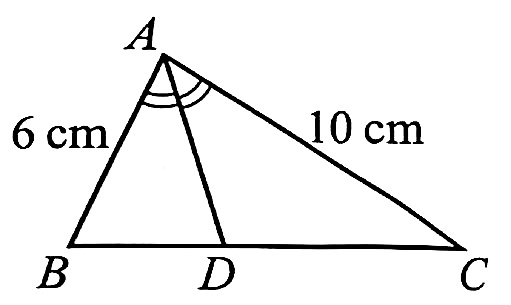
\includegraphics[width=0.25\textwidth]{assets/10-33.jpg}
        \end{vwcol}
    }

    \vspace{3em}
    \item \parbox[t]{0.9\textwidth}{
        ~
        \vspace{-1.1em}
        \begin{vwcol}[widths={0.7,0.3}, sep=8mm, rule=0pt]
            In triangle $PQR$, $PQ = 16$, $PR = 13$, $QS = 8$. If $S$ is a point on segment $QR$ and $PS = 12$, find $\angle PRS$.
    
            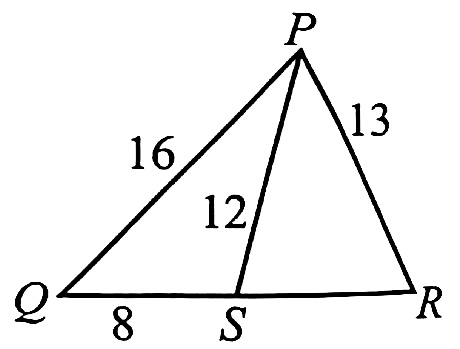
\includegraphics[width=0.23\textwidth]{assets/10-34.jpg}
        \end{vwcol}
    }
    \end{enumerate}

    \vspace{1em}
    \subsection*{Given Two Sides and Their Included Angle of a Triangle, Find the Area}

    \vspace{-1em}
    \begin{center}
        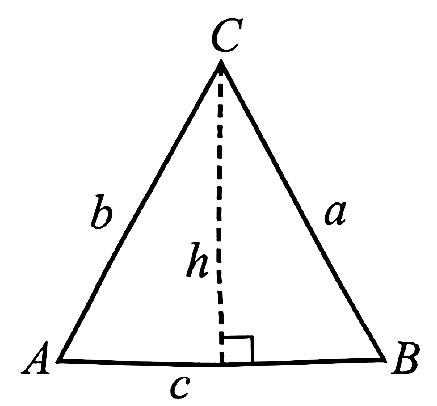
\includegraphics[width=0.2\textwidth]{assets/10-35.jpg}
        \hspace{3em}
        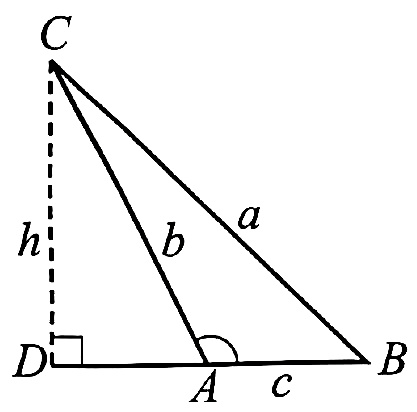
\includegraphics[width=0.2\textwidth]{assets/10-36.jpg}
        \hspace{3em}
        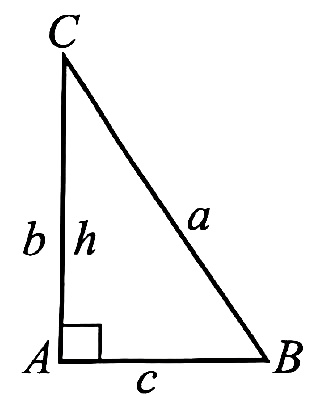
\includegraphics[width=0.16\textwidth]{assets/10-37.jpg}
    \end{center}

    \vspace{-1em}
    As shown in figures above, considering acute, obtuse, and right-angled triangles. In triangle $ABC$, let $h$ be the height drawn from side $AB$. 
    
    If $\angle A$ is acute, then $h = b \sin A$.

    If $\angle A$ is obtuse, then $h = b \sin (180^\circ - A) = b \sin A$.

    If $\angle A$ is right, since $\sin A = \sin 90^\circ = 1$, then $h = b = b \sin A$.

    This means that regardless of whether triangle $ABC$ is acute, obtuse, or right-angled, we have the relationship $h = b \sin A$. Therefore,
    $$
    \text{Area of triangle } ABC = \Delta = \dfrac{1}{2}ch = \dfrac{1}{2}bc\sin A
    $$

    \vspace{-1em}
    Similarly, it can be proved that
    $$
    \Delta = \dfrac{1}{2}ca\sin B, \quad \Delta = \dfrac{1}{2}ab\sin C
    $$

    \vspace{-1em}        
    In this chapter, the area of a triangle will be denoted by $\Delta$.

    From this, we can see that given the two sides and their included angle, the formula for the area of triangle $ABC$ is

    \begin{info}[Area of a Triangle]
        $$
        \Delta = \dfrac{1}{2}ab\sin C = \dfrac{1}{2}bc\sin A = \dfrac{1}{2}ca\sin B
        $$
    \end{info}

    We can derive another proof of the law of sine based on the formula for the area of a triangle. From the formula for the area of a triangle:
    $$
    \dfrac{1}{2}bc\sin A = \dfrac{1}{2}ca\sin B = \dfrac{1}{2}ab\sin C
    $$

    \vspace{-1em}
    Dividing all sides of the equation by $\dfrac{1}{2}abc$, we get
    $$
    \dfrac{\sin A}{a}=\dfrac{\sin B}{b}=\dfrac{\sin C}{c} \Rightarrow \dfrac{a}{\sin A}=\dfrac{b}{\sin B}=\dfrac{c}{\sin C}
    $$

    \vspace{-1em}
    This is the law of sines.

    \begin{question}
        Find the area of the following $\triangle ABC$.
        \vspace{-1em}
        \begin{enumerate}[label=(\alph*)]
            \item $a=20 \mathrm{~cm}, b=35 \mathrm{~cm}, C=105^{\circ}$
            \item $A=36^{\circ}, c=20 \mathrm{~cm}, C=85^{\circ}$
        \end{enumerate}

        \sol{}
        \begin{enumerate}[label=(\alph*)]
            \item \parbox[t]{0.9\textwidth}{
                ~
                \vspace{-1.3em}
                \begin{vwcol}[widths={0.7,0.3}, sep=8mm, rule=0pt]
                    Using the formula $\Delta=\dfrac{1}{2}ab\sin C$, we get 
            
            \noindent $\Delta=\dfrac{1}{2} \times 20 \times 35 \times \sin 105^{\circ}=338.07 \mathrm{~cm}^{2}$.

            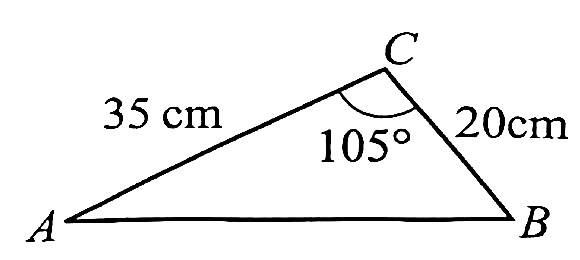
\includegraphics[width=0.25\textwidth]{assets/10-38.jpg}
                \end{vwcol}
            }

            \item \parbox[t]{0.9\textwidth}{
                ~
                \vspace{-1.1em}
                \begin{vwcol}[widths={0.7,0.3}, sep=8mm, rule=0pt]
                    $B = 180^\circ - 36^\circ - 85^\circ = 59^\circ$. 
            
                    \noindent Using the law of sine, we get $\dfrac{a}{\sin 36^\circ} = \dfrac{20}{\sin 85^\circ}$.

                    \noindent $\therefore$ $a = \dfrac{20}{\sin 85^\circ} \times \sin 36^\circ = 11.80$

                    \noindent Using the formula $\Delta = \dfrac{1}{2}ac\sin B$, we get 
                    
                    \noindent $\Delta = \dfrac{1}{2} \times 20 \times 11.80 \times \sin 59^\circ = 101.15 \mathrm{~cm}^{2}$.

                    \vspace{3em}
                    \parbox{0.25\textwidth}{
                    \vspace{3em}
                    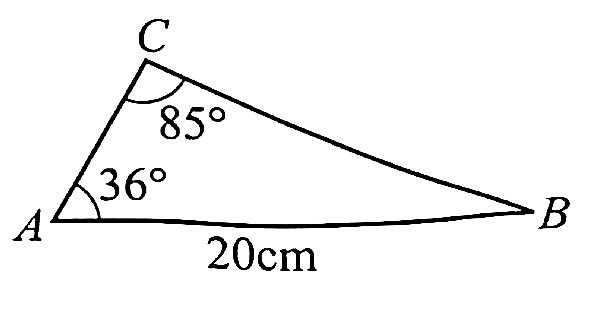
\includegraphics[width=0.25\textwidth]{assets/10-39.jpg}}
                \end{vwcol}
            }
            \vspace{-5em}
        \end{enumerate}
    \end{question}

    \begin{question}
        Given that n $\triangle ABC$, $AB = 3 \mathrm{~cm}$ and $AC = 6 \mathrm{~cm}$, find the maximum area of triangle $ABC$.

        \sol{}
        \begin{vwcol}[widths={0.6,0.4}, sep=8mm, rule=0pt,justify=flushleft]
            \noindent Using the formula $\Delta = \dfrac{1}{2}bc\sin A$, we get 
        
            \noindent $\begin{aligned} & \Delta=\dfrac{1}{2} \times 6 \times 3 \times \sin A=9 \sin A \\ & \because-1 \leq \sin A \leq 1 \\ & \therefore \Delta=9 \sin A \leq 9\end{aligned}$

            \noindent Hence, the maximum area of $\triangle ABC$ is $9 \mathrm{~cm}^{2}$.
            \vspace{3em}

            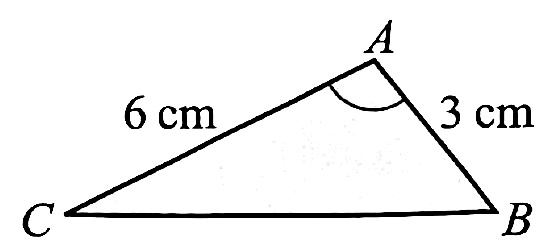
\includegraphics[width=0.25\textwidth]{assets/10-40.jpg}
        \end{vwcol}
        \vspace{-1em}    
    \end{question}

    \vspace{-1em}    
    \begin{think}
        
        \noindent In Example 11, what kind of triangle is $\triangle ABC$ when the area is maximized?
    \end{think}

    \practice{10.3a}
    \vspace{-1em}
    \begin{vwcol}[widths={0.7,0.3}, sep=8mm, rule=0pt]
        \parbox{0.7\textwidth}{
        \begin{enumerate}
        \item Find the area of triangle $ABC$ in the figure.

        \item In triangle $PQR$, where $QR = 10 \mathrm{~cm}$ and $\angle Q = 60^\circ$, if the area of triangle $PQR$ is $10 \sqrt{3} \mathrm{~cm}^{2}$, find:
        \begin{enumerate}
            \item the length of $PR$;
            \item $\angle P$.
        \end{enumerate}
    \end{enumerate}}
    
    \vspace{-5em}
    \parbox{0.3\textwidth}{
        \vspace{1em}
        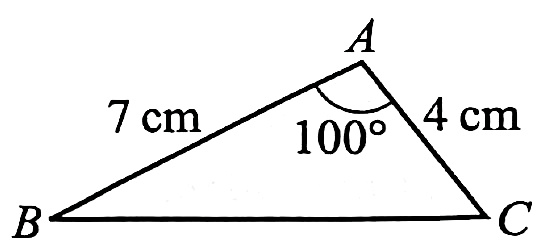
\includegraphics[width=0.25\textwidth]{assets/10-41.jpg}
    }
    \end{vwcol}

    \vspace{-1em}
    \subsection*{Given Three Sides of a Triangle, Find the Area}

    \vspace{-1em}
    Consider an arbitrary $\triangle ABC$, from the law of cosine, we have $\cos C = \dfrac{a^2 + b^2 - c^2}{2ab}$. Hence,
    \begin{flalign*}
        \sin C & =\dfrac{\sqrt{(2 a b)^2-\left(a^2+b^2-c^2\right)^2}}{2 a b} \\ & =\dfrac{\sqrt{(a+b+c)(a+b-c)(a-b+c)(b+c-a)}}{2 a b} &
    \end{flalign*}

    \vspace{-1.5em}
    \begin{vwcol}[widths={0.6,0.4}, sep=8mm, rule=0pt]
        ~
        
        \vspace{-1.1em}
        Let $s = \dfrac{1}{2}(a + b + c)$. The above expression can be rewritten as:
    \begin{align*}
        \sin C = \dfrac{2}{ab} \sqrt{s(s - a)(s - b)(s - c)}
    \end{align*}

    \vspace{-1em}
    We can rewrite $\Delta = \dfrac{1}{2}ab\sin C$ as:
    \begin{align*}
        \Delta &= \dfrac{1}{2}ab \cdot \dfrac{2}{ab} \sqrt{s(s - a)(s - b)(s - c)} \\
        &= \sqrt{s(s - a)(s - b)(s - c)}
    \end{align*}
    \vspace{3em}

    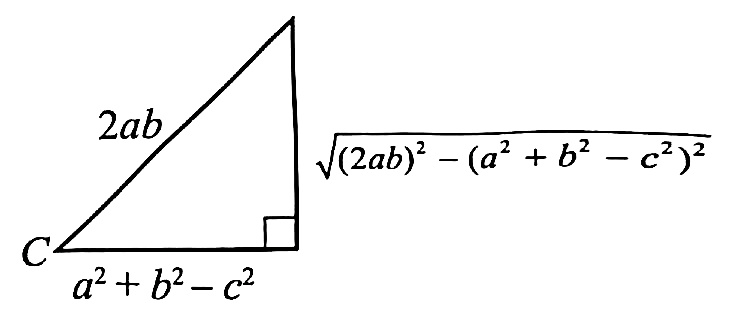
\includegraphics[width=0.35\textwidth]{assets/10-42.jpg}
    \end{vwcol}

    From this, we can see that given the three sides of a triangle, the formula for the area of triangle $ABC$ is
    
    \begin{info}[Heron's Formula]
        $$
        \Delta = \sqrt{s(s - a)(s - b)(s - c)}, \text{ where } s = \dfrac{1}{2}(a + b + c)
        $$
    \end{info}

    \begin{question}
        Given that the three sides of triangle $ABC$ are $41 \mathrm{~cm}$, $425 \mathrm{~cm}$, and $416 \mathrm{~cm}$, find the area of this triangle.

        \sol{}

        \begin{vwcol}[widths={0.6,0.4}, sep=8mm, rule=0pt,justify=flushleft]
            \noindent From $s=\dfrac{1}{2}(41+416+425)=441$,

        \noindent Substituting into Heron's formula $\Delta=\sqrt{s(s-a)(s-b)(s-c)}$, we get 
        
        \vspace{0.5em}
        \noindent $\begin{aligned} \Delta & =\sqrt{441(441-41)(441-416)(441-425)} \\ & =8400 \mathrm{~cm}^2\end{aligned}$

        \vspace{3em}
        
        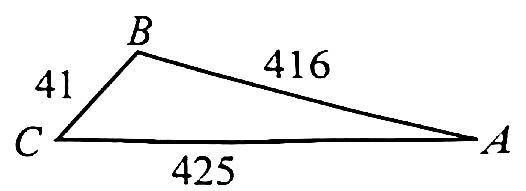
\includegraphics[width=0.3\textwidth]{assets/10-43.jpg}
        \end{vwcol}
        \vspace{-1em}
    \end{question}

    \practice{10.3b}
    \begin{vwcol}[widths={0.7,0.3}, sep=8mm, rule=0pt]
        As shown in the figure, in quadrilateral $ABCD$, $AB = 4$, $BC = 14$, $CD = 6$, $BD = 10$, and $\angle ABD = 60^\circ$. Find the area of quadrilateral $ABCD$.

        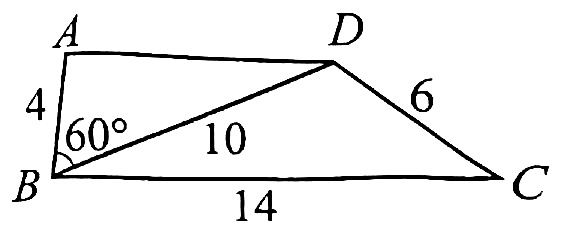
\includegraphics[width=0.27\textwidth]{assets/10-44.jpg}
    \end{vwcol}

    \exercise{10.3}
    \begin{enumerate}
        \item \parbox[t]{0.9\textwidth}{
            ~
            \vspace{-1.1em}
            \begin{vwcol}[widths={0.7,0.3}, sep=8mm, rule=0pt]
                Find the area of triangle $PQR$ in the figure on the right.
    
                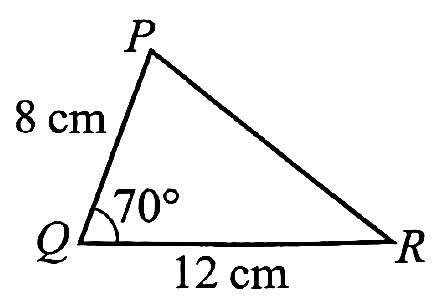
\includegraphics[width=0.23\textwidth]{assets/10-45.jpg}
            \end{vwcol}
        }
        
        \vspace{4em}
        \item \parbox[t]{0.9\textwidth}{
            ~
            \vspace{-1.1em}
            \begin{vwcol}[widths={0.7,0.3}, sep=8mm, rule=0pt]
                If the area of the triangle in the right figure is $21 \sqrt{2} \mathrm{~cm}^{2}$, and $DE = 12 \mathrm{~cm}$, $\angle FED = 45^\circ$, find the length of $EF$.
    
                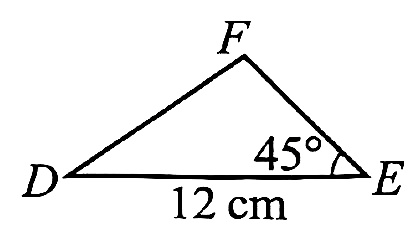
\includegraphics[width=0.2\textwidth]{assets/10-46.jpg}
            \end{vwcol}
        }
        
        \vspace{3em}
        \item \parbox[t]{0.9\textwidth}{
            ~
            \vspace{-1.1em}
            \begin{vwcol}[widths={0.7,0.3}, sep=8mm, rule=0pt]
                As shown in the figure on the right, an umbrella canopy is made up of ten equal isosceles triangles of side lengths $50 \mathrm{~cm}$, $50 \mathrm{~cm}$, and $20 \mathrm{~cm}$. Find the area of waterproof fabric needed to make one umbrella.
    
                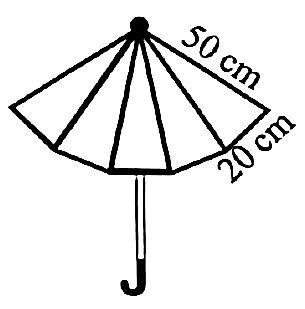
\includegraphics[width=0.18\textwidth]{assets/10-47.jpg}
            \end{vwcol}
        }
        
        \item In triangle $ABC$, where $A = 45^\circ$, $AB = 3 \mathrm{~cm}$, and $BC = \sqrt{6} \mathrm{~cm}$, find the area of triangle $ABC$.
        
        \item \parbox[t]{0.9\textwidth}{
            ~
            \vspace{-1.1em}
            \begin{vwcol}[widths={0.7,0.3}, sep=8mm, rule=0pt]
                In the right figure, $OACB$ is a sector. Find the area of the shape $ACB$.
    
                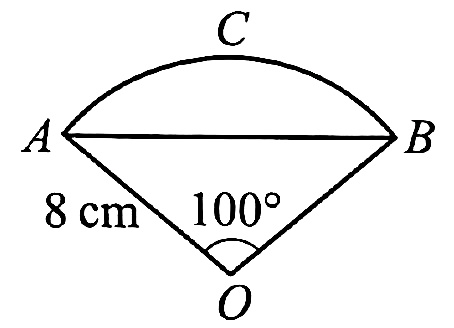
\includegraphics[width=0.2\textwidth]{assets/10-48.jpg}
            \end{vwcol}
        }
        
        \vspace{3em}
        \item \parbox[t]{0.9\textwidth}{
            ~
            \vspace{-1.1em}
            \begin{vwcol}[widths={0.7,0.3}, sep=8mm, rule=0pt]
                In the right figure, $AD$ is the altitude from side $BC$, $AD = h$.
        
                \noindent Express $AB$, $CA$, $BC$, and the area of $\triangle ABC$ in terms of $h$.
                
                \noindent Hence, prove that $\sin 75^\circ = \dfrac{\sqrt{6} + \sqrt{2}}{4}$.
    
                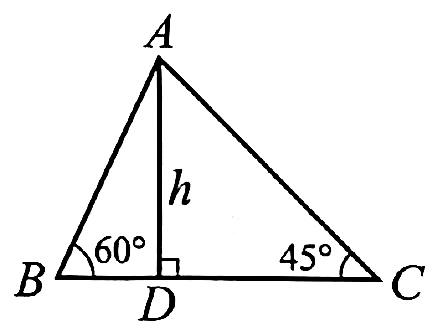
\includegraphics[width=0.2\textwidth]{assets/10-49.jpg}
            \end{vwcol}
        }

        \item \parbox[t]{0.9\textwidth}{
            ~
            \vspace{-1.1em}
            \begin{vwcol}[widths={0.7,0.3}, sep=8mm, rule=0pt]
                In triangle $ABC$, where $AB = 12$, $AC = 6$, and $\angle BAC = 60^\circ$, if the angle bisector of $\angle BAC$ intersects $BC$ at point $D$, find the length of $AD$.
    
                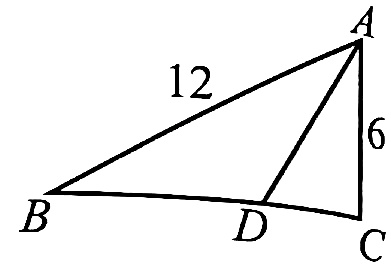
\includegraphics[width=0.2\textwidth]{assets/10-50.jpg}
            \end{vwcol}
        }

        \vspace{3em}
        \item Honeycomb cardboard is made based on the natural structure of honeycombs. The core of the honeycomb cardboard is formed by corrugated paper, and the cross-section of this hollow cylinder is a regular hexagon. This structure gives the cardboard excellent cushioning performance. Given that the side length of the hexagonal base is $6 \mathrm{~mm}$ and the height is $10 \mathrm{~mm}$, find the volume of this cylinder.
        \begin{center}
            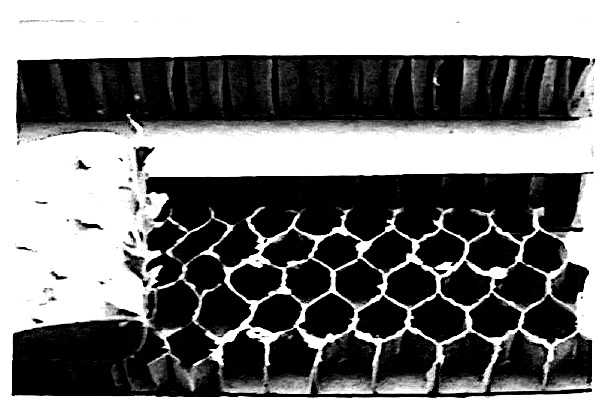
\includegraphics[width=0.3\textwidth]{assets/10-51.jpg}
            \hspace{3em}
            \includegraphics[width=0.2\textwidth]{assets/10-52.jpg}
            \hspace{3em}
            \includegraphics[width=0.18\textwidth]{assets/10-53.jpg}
        \end{center}

        \item \parbox[t]{0.9\textwidth}{
            ~
            \vspace{-1.1em}
            \begin{vwcol}[widths={0.7,0.3}, sep=8mm, rule=0pt]
                The figure shows the field and dormitory of Chong Hua High School, Kluang. Given that region $ABCD$ is a trapezoid where $BC \parallel AD$, and the lengths of the sides are $207 \mathrm{~m}$, $158 \mathrm{~m}$, $162 \mathrm{~m}$, and $165 \mathrm{~m}$, find the area of $ABCD$.
    
                \includegraphics[width=0.3\textwidth]{assets/10-54.jpg}
            \end{vwcol}
        }

    \vspace{4em}
    \item In triangle $ABC$, if $a:b:c = 4\sqrt{2}:5:7$ and the radius of the circumcircle is $10\sqrt{2} \mathrm{~cm}$, find the area of triangle $ABC$.
    \end{enumerate}

    \newpage
    \section{Problems Related to Measurement}

    \vspace{-1em}
    In this section, we will use the law of sine and the law of cosine to solve some relatively complex application problems.

    \vspace{-1em}
    \subsection*{Angle of Elevation and Depression}
    \vspace{-1em}
    \begin{center}
        \includegraphics[width=0.5\textwidth]{assets/10-55.jpg}
    \end{center}

    \vspace{-1.5em}    
    In practical measurement problems, we often encounter terms like "angle of elevation" and "angle of depression." For example, when looking from the top of a hill to the top and bottom of a tree, the lines of sight to the top and bottom of the tree form angles with the horizontal line. We call $\alpha$ the angle of elevation and $\beta$ the angle of depression.

    \begin{question}
       \begin{vwcol}[widths={0.6,0.4}, sep=8mm, rule=0pt]
             As shown in the figure, from two points $A$ and $B$ on the ground, the angle of elevation to the top $C$ of the Leaning Tower of Pisa is measured to be $80^\circ$ and $72^\circ$ respectively. It is known that point $A$ is $15.27 \mathrm{~m}$ away from the center point $D$ of the tower base, and $AB$ is $8.32 \mathrm{~m}$ apart. Find the height of the tower $CD$ and the inclination.

            \includegraphics[width=0.25\textwidth]{assets/10-56.jpg}
        \end{vwcol}

        \sol{}
        
        \begin{vwcol}[widths={0.6,0.4}, sep=8mm, rule=0pt,justify=flushleft]
            \noindent In $\triangle ABC$, $\angle ACB = 80^\circ - 72^\circ = 8^\circ$.
        
            \noindent Using the law of sines, we have $\dfrac{AC}{\sin 72^\circ} = \dfrac{8.32}{\sin 8^\circ}$.
            
            \noindent $
            \therefore AC = \dfrac{8.32 \sin 72^\circ}{\sin 8^\circ} = 56.8557
            $

            \vspace{1em}
            \noindent In triangle $ACD$, using the law of cosines, we have
                
            \vspace{1em}
            \noindent $
            \begin{aligned}
            CD^2 & = AD^2 + AC^2 - 2 \times AD \times AC \times \cos 80^\circ \\
            & = 15.27^2 + 56.8557^2 - 2 \times 15.27 \times 56.8557 \times \cos 80^\circ \\
            \therefore CD & = 56.2514 \mathrm{~m}
            \end{aligned}
            $

            \noindent From the law of sines, we have $\begin{aligned}[t] \dfrac{A C}{\sin \angle A D C} & =\dfrac{C D}{\sin 80^{\circ}} \\ \sin \angle A D C & =\dfrac{A C \sin 80^{\circ}}{C D} \\ & =\dfrac{56.8557 \sin 80^{\circ}}{56.2514}\end{aligned}$

            \vspace{5em}

            \includegraphics[width=0.23\textwidth]{assets/10-1.jpg}
        \end{vwcol}
        \vspace{-2em}
        \noindent Since $\angle ADC$ is an acute angle, $\angle ADC = 84.49^\circ$.

        \vspace{-0.8em}
        \noindent Therefore, the inclination of the Tower $= 90^\circ - 84.49^\circ = 5.51^\circ$.

        \vspace{-0.8em}
        \noindent Hence, the height of the Leaning Tower of Pisa $CD$ is $56.25 \mathrm{~m}$, and the inclination is $5.51^\circ$.
    \end{question}

    \begin{question}
        \begin{vwcol}[widths={0.6,0.4}, sep=8mm, rule=0pt]
            A communication satellite $S$ orbits the Earth and passes over two ground stations $A$ and $B$ on the equator. If these two ground stations are $100$ km apart and the elevation angles measured from satellite $S$ to stations $A$ and $B$ are $83^\circ$ and $86^\circ$ respectively, at the same moment, how many milliseconds does it take for an electromagnetic wave signal to be transmitted from satellite $S$ to station $B$, given that the speed of electromagnetic waves is $3 \times 10^8$ m/s?
            
            \includegraphics[width=0.3\textwidth]{assets/10-57.jpg}
        \end{vwcol}

        \sol{}
        \begin{vwcol}[widths={0.6,0.4}, sep=8mm, rule=0pt,justify=flushleft]
            \noindent Let $C$ be the foot of the perpendicular from satellite $S$ to the Earth's surface.

            \noindent In $\triangle ABS$, $\angle ASB = 86^\circ - 83^\circ = 3^\circ$.

            \vspace{1em}
            \noindent Using the law of sines, we have $\dfrac{BS}{\sin 83^\circ} = \dfrac{100}{\sin 3^\circ}$.

            \noindent $
            BS = \dfrac{100}{\sin 3^\circ} \times \sin 83^\circ = 1896.49
            $

            \vspace{1em}
            \noindent Since the distance between ground station $B$ and satellite $S$ is $1896.49$ km,

            \noindent the time taken for an electromagnetic wave signal to be transmitted from satellite $S$ to station $B$ is

            \vspace{1em}
            \noindent $
            \dfrac{1896.49 \times 1000 \mathrm{~m}}{3 \times 10^8 \mathrm{~m} / \mathrm{s}} = 6.32 \times 10^{-3} \mathrm{~s} = 6.32 \text{ milliseconds}.
            $

            \vspace{10em}
            \includegraphics[width=0.23\textwidth]{assets/10-58.jpg}
        \end{vwcol}
    \end{question}

    \practice{10.4a}
    \begin{enumerate}
        \item \parbox[t]{0.9\textwidth}{
            ~
            \vspace{-1.1em}
            \begin{vwcol}[widths={0.6,0.4}, sep=8mm, rule=0pt]
                As shown in the figure on the right, the elevation angles of the top of the KL Tower $R$ from two points $P$ and $Q$ on the ground are $57^\circ$ and $70^\circ$ respectively. Given that the distance between $P$ and $Q$ is $120$ m, find the height of the KL Tower.
    
                \includegraphics[width=0.16\textwidth]{assets/10-59.jpg}
            \end{vwcol}
        }

        \vspace{3em}
        \item \parbox[t]{0.9\textwidth}{
            ~
            \vspace{-1.1em}
            \begin{vwcol}[widths={0.6,0.4}, sep=8mm, rule=0pt]
                As shown in the figure on the right, the angle of depression from the top $K$ of an observation tower to a point $L$ on the ground is $63^\circ$. If we move $25$ m down from $K$ to point $M$, the angle of depression to $L$ becomes $55^\circ$. Find the distance between the observation tower and point $L$.
    
                \includegraphics[width=0.25\textwidth]{assets/10-60.jpg}
            \end{vwcol}
        }
    \end{enumerate}
    
    \newpage
    \begin{explore}[Exploration Activity 1]

    \begin{enumerate}[label=\textbf{Aim: }, leftmargin=*]
        \item To actually measure the height of a lamppost and understand the practical applications of trigonometry in daily life.
    \end{enumerate}

    \vspace{-2em}
    \begin{enumerate}[label=\textbf{Tool: }, leftmargin=*]
        \item Watch the video and learn how to make and operate a clinometer for measurements. 
    
        \url{https://youtu.be/FVqNEBWH4B0}
    \end{enumerate}   

    \vspace{-2em}
    \begin{enumerate}[label=\textbf{Control Variables: }, leftmargin=*]
        \item Height of the lamppost $H$, height of the measurer $h$.
    \end{enumerate}

    \vspace{-2em}
    \begin{enumerate}[label=\textbf{Manipulated Variables: }, leftmargin=*]
        \item Horizontal distance between the measurer and the lamppost $x$, angle of elevation $\theta$ observed by the measurer to the top of the lamppost.
    \end{enumerate}

    \vspace{-2em}
    \begin{enumerate}[label=\textbf{Procedure: }, leftmargin=*]
        \item Draw a simple figure and list the process for calculating the height $H$ of a lamppost.
        \begin{center}
            \includegraphics[width=0.35\textwidth]{assets/10-62.jpg}
            \hspace{3em}
            \includegraphics[width=0.2\textwidth]{assets/10-61.jpg}
        \end{center}
    \end{enumerate}

    \noindent\textbf{Discuss the Results:} 
    \vspace{-1em}
    \begin{enumerate}[leftmargin=*]
        \item  What difficulties occurred during the observation? How were they resolved? Are there any unresolved issues?

        \item Is the calculation process based on specific assumptions? If so, please specify.

        \item Are there any factors that may affect the calculation results?
    \end{enumerate}

    \noindent \textbf{Extended Discussion:}

    \noindent Assuming the observed object is a mountain, it is often difficult in practice to measure the vertical distance from the mountaintop to the ground. With reference to the figure below, can you utilize the two measured angles of elevation $\alpha$ and $\beta$ and the distance $d$ between the two observation points to represent the height $h$ of the mountain?
    \begin{center}
        \includegraphics[width=0.5\textwidth]{assets/10-63.jpg}
    \end{center}
    \end{explore}

    \newpage

    \subsection*{Bearings}

    \begin{vwcol}[widths={0.7,0.3}, sep=8mm, rule=0pt]
        In surveying, the \textbf{bearing} is commonly used to measure the direction of a target relative to the survey point. When using bearings, all directions are measured clockwise from true north to the target point $P$, which is referred to as the bearing of $P$ from $O$. The bearing must be written in three-digit form, with values ranging from $000^\circ$ to $360^\circ$.

        \includegraphics[width=0.2\textwidth]{assets/10-64.jpg}
    \end{vwcol}

   \begin{vwcol}[widths={0.7,0.3}, sep=8mm, rule=0pt]
         For example, in the diagram on the right, the bearing measured
    
    \noindent from $O$ to $A$ is $070^\circ$, 
    
    \noindent from $O$ to $B$ is $150^\circ$, 
    
    \noindent from $O$ to $C$ is $270^\circ$, 
    
    \noindent from $O$ to $D$ is $310^\circ$.

    \includegraphics[width=0.23\textwidth]{assets/10-65.jpg}
   \end{vwcol}

   \begin{question}
    \begin{vwcol}[widths={0.7,0.3}, sep=8mm, rule=0pt]
        A cargo ship is sailing at a speed of 35 nautical miles per hour along a bearing of $148^\circ$. At point $B$, the cargo ship observes the bearing of lighthouse $A$ to be $126^\circ$. After sailing for half an hour, it reaches point $C$ and observes the bearing of lighthouse $A$ to be $078^\circ$. Find the distance between the cargo ship at point $C$ and lighthouse $A$.

        \vspace{2em}    
        \sol{}
        \vspace{1em}
        
        \noindent $
        \begin{aligned}
        & \text{In triangle } ABC, BC = \dfrac{1}{2} \times 35 = 17.5 \\
        & \angle ABC = 148^\circ - 126^\circ = 22^\circ
        \end{aligned}
        $
        
        \vspace{1em}
        \noindent Since $DB \parallel EC$, by alternate interior angles, $\angle ECB + 148^\circ = 180^\circ$.
        
        \vspace{0.8em}
        \noindent $\therefore \angle ECB = 32^\circ$

        \vspace{4em}

        \includegraphics[width=0.25\textwidth]{assets/10-66.jpg}
    \end{vwcol}
    \vspace{-2.3em}
    \noindent Hence, $\angle A C B=32^{\circ}+78^{\circ}=110^{\circ}$

    \vspace{-0.5em}
    \noindent $
    \angle B A C=180^{\circ}-\angle A B C-\angle A C B=180^{\circ}-22^{\circ}-110^{\circ}=48^{\circ}
    $

    \vspace{-0.5em}
    \noindent By the law of sines, we have $\dfrac{AC}{\sin 22^\circ} = \dfrac{17.5}{\sin 48^\circ}$.
    
    \vspace{-0.5em}
    \noindent $
    AC = 17.5 \times \dfrac{\sin 22^\circ}{\sin 48^\circ} = 8.82 \text{ nautical miles}.
    $
    
    \vspace{-0.5em}
    \noindent Hence, the distance between the cargo ship at point $C$ and lighthouse $A$ is $8.82$ nautical miles.
   \end{question}

   \begin{info}[Nautical Mile]
    A nautical mile is a unit of length used in air and marine navigation.
    $$1 \text{ nautical mile} \approx 1.852 \text{ km}$$
    \end{info}

    \newpage
    \begin{question}
        A destroyer receives intelligence that an enemy ship is located $10$ nautical miles away in the direction of $036^\circ$. The enemy ship is sailing at a speed of $16$ nautical miles per hour along a bearing of $104^\circ$. Given that the destroyer's speed is $21$ nautical miles per hour, find the bearing $x^\circ$ and the time $t$ in hours it takes for the destroyer to intercept the enemy ship.

        \sol{}
        
        \begin{vwcol}[widths={0.7,0.3}, sep=8mm, rule=0pt,justify=flushleft]
            \noindent Let the initial position of the destroyer be at point $A$ and the initial position of the enemy ship be at point $B$, where they meet at point $C$. 
        
            \vspace{0.5em}
            \noindent We have $AB = 10$ nautical miles, $BC = 16t$ nautical miles, and $AC = 21t$ nautical miles.
            
            \vspace{0.5em}
            \noindent The relationship can be drawn as shown on the right.

            \vspace{0.5em}
            \noindent In $\triangle ABC$, we have $\angle ABC = 36^\circ + (180^\circ - 104^\circ) = 112^\circ$.
            
            \includegraphics[width=0.25\textwidth]{assets/10-67.jpg} 
        \end{vwcol}
        
        \vspace{-3em}
        \noindent Using the law of cosines, we get:
        \begin{flalign*}
            cos 112^\circ &= \dfrac{10^2 + (16t)^2 - (21t)^2}{2 \times 10 \times 16t} &\\
        \cos 112^\circ &= \dfrac{100 - 185t^2}{320t}
        \end{flalign*}
        Rearranging, we have:
        \begin{flalign*}
            & 185t^2 + (320 \cos 112^\circ)t - 100 = 0 &\\
            &t = \dfrac{-320 \cos 112^\circ \pm \sqrt{(320 \cos 112^\circ)^2 - 4 \times 185 \times (-100)}}{2 \times 185}\\
            &t = 1.13 \text{ or } t = -0.48 \text{ (rejected)}
        \end{flalign*}

        \vspace{-1.5em}
        \noindent Also, using the law of cosines, we get:
        \vspace{-0.5em}

        \noindent $
        \cos \angle BAC = \dfrac{10^2 + (21t)^2 - (16t)^2}{2 \times 10 \times 21t} = \dfrac{100 + 185t^2}{420t}
        $

        \vspace{-0.5em}
        \noindent Substituting the obtained value of $t$, we can find $\angle BAC = 44.9^\circ$.
        
        \vspace{-0.5em}
        \noindent $
        x^\circ = 036^\circ + 044.9^\circ = 080.9^\circ
        $

        \vspace{-0.5em}
        \noindent Therefore, $x$ equals $080.9$ and $t$ equals $1.13$.
    \end{question}

    \practice{10.4b}

    There are two docks, $A$ and $B$. Ship $A$ departs from dock $A$ at a speed of $40$ nautical miles per hour in the direction of $070^\circ$. Ship $B$ departs from dock $B$ at a speed of $50$ nautical miles per hour in the direction of $220^\circ$. If both ships arrive at point $C$ simultaneously after $45$ minutes, find the distance between the two docks.

    \newpage
    \exercise{10.4}
    \begin{enumerate}
        \item \parbox[t]{0.9\textwidth}{
            ~
            \vspace{-1.1em}
            \begin{vwcol}[widths={0.6,0.4}, sep=8mm, rule=0pt]
                Xiao Hua observes the elevation angle of the top of the Eiffel Tower, $L$, from point $M$ on the ground as $70^\circ$. After walking forward $48.5 \mathrm{~m}$ to point $K$, she observes the elevation angle of the top of the tower as $78^\circ$. Find the height of the Eiffel Tower.
    
                \includegraphics[width=0.25\textwidth]{assets/10-68.jpg}
            \end{vwcol}
        }

        \vspace{3em}
        \item \parbox[t]{0.9\textwidth}{
            ~
            \vspace{-1.1em}
            \begin{vwcol}[widths={0.6,0.4}, sep=8mm, rule=0pt]
                In the diagram on the right, there's an inclined utility pole. Xiao Ming stands at point $A$, $2 \mathrm{~m}$ away from the pole, and measures the elevation angle of the top of the pole as $83^\circ$. He steps back $3 \mathrm{~m}$ to point $B$, where he measures the elevation angle of the top of the pole as $70^\circ$. Find the length and inclination of the utility pole.
    
                \includegraphics[width=0.25\textwidth]{assets/10-69.jpg}
            \end{vwcol}
        }

        \vspace{2em}    
        \item \parbox[t]{0.9\textwidth}{
            ~
            \vspace{-1.1em}
            \begin{vwcol}[widths={0.6,0.4}, sep=8mm, rule=0pt]
                As shown in the diagram on the right, a communication tower stands at the top of a slope with a gradient of $67^\circ$. If a cable is to be pulled from above the communication tower to a point $165 \mathrm{~m}$ in front of the communication tower, and the angle between the cable and the slope is $16^\circ$, find the length of this cable.
    
                \includegraphics[width=0.25\textwidth]{assets/10-71.jpg}
            \end{vwcol}
        }

        \vspace{3em}
        \item \parbox[t]{0.9\textwidth}{
            ~
            \vspace{-1.1em}
            \begin{vwcol}[widths={0.6,0.4}, sep=8mm, rule=0pt]
                a ship on the sea is observed from the edge of a cliff with a depression angle of $60^\circ$. After the ship sails $45 \mathrm{~m}$ away from the cliff, the elevation angle from the edge of the cliff becomes $35^\circ$. Find the height of the cliff above the sea level.
    
                \includegraphics[width=0.3\textwidth]{assets/10-70.jpg}
            \end{vwcol}
        }

        \vspace{4em}
        \item \parbox[t]{0.9\textwidth}{
            ~
            \vspace{-1.1em}
            \begin{vwcol}[widths={0.6,0.4}, sep=8mm, rule=0pt]
                A ship observes the bearing of lighthouse $C$ from dock $A$ as $060^\circ$. The ship departs from dock $A$ at a speed of $40$ nautical miles per hour and heads east. After sailing for $2$ hours, it arrives at dock $B$, where the bearing of lighthouse $C$ is measured as $340^\circ$. Find the distance between dock $B$ and lighthouse $C$.
    
                \includegraphics[width=0.3\textwidth]{assets/10-72.jpg}
            \end{vwcol}
        }

        \newpage    
        \item \parbox[t]{0.9\textwidth}{
            ~
            \vspace{-1.1em}
            \begin{vwcol}[widths={0.6,0.4}, sep=8mm, rule=0pt]
                Two ships, $A$ and $B$, depart simultaneously from dock $O$. Ship $A$ sails at a speed of $45$ nautical miles per hour in the direction of $150^\circ$, while ship $B$ sails at a speed of $54$ nautical miles per hour in the direction of $110^\circ$. After three hours, find:
                
                \noindent\parbox[t]{0.5\textwidth}{
                    \begin{enumerate}
                        \item the distance between ship $A$ and ship $B$;
                        \item the bearing of ship $B$ as observed from ship $A$. (Round to the nearest degree)
                    \end{enumerate}
                }
    
                \includegraphics[width=0.26\textwidth]{assets/10-73.jpg}
            \end{vwcol}
        }

        \vspace{-3em}
        \item \parbox[t]{0.9\textwidth}{
            ~
            \vspace{-1.1em}
            \begin{vwcol}[widths={0.6,0.4}, sep=8mm, rule=0pt]
                A ship sails from dock $P$ towards the east at a speed of 50 nautical miles per hour, reaching island $K$ after $45$ minutes. Then, it continues sailing towards northeast and arrives at island $L$ after one hour. We need to find:
        
                \noindent\parbox[t]{0.5\textwidth}{
                    \begin{enumerate}
                        \item the distance between dock $P$ and island $L$;
                        \item the bearing of island $L$ as observed from dock $P$. (Round to the nearest degree)
                    \end{enumerate}
                }
    
                \includegraphics[width=0.3\textwidth]{assets/10-74.jpg}
            \end{vwcol}
        }
    \end{enumerate}

    \revision{10}
    \begin{enumerate}
        \item Given that the ratio of the three sides of triangle $\triangle PQR$ is $PQ:QR:PR=9:5:7$, find its smallest internal angle.
        \item If the ratios of the three interior angles of triangle $\triangle PQR$ are $\angle P:\angle Q:\angle R=7:3:8$ and $PQ=24 \mathrm{~cm}$, find the length of the shortest side.
        \item Given in triangle $\triangle ABC$, $AB=6 \mathrm{~cm}$, $BC=8 \mathrm{~cm}$, and the area of triangle $\triangle ABC$ is $20 \mathrm{~cm}^2$, find $\angle B$.
        \item \parbox[t]{0.9\textwidth}{
            ~
            \vspace{-1.1em}
            \begin{vwcol}[widths={0.6,0.4}, sep=8mm, rule=0pt]
                In the figure on the right, if the sides of the triangle satisfy the relation: $(a+b):(b+c):(a+c)=5:6:7$, find $\angle A$.
    
                \includegraphics[width=0.25\textwidth]{assets/10-75.jpg}
            \end{vwcol}
        }

        \vspace{3em}
        \item \parbox[t]{0.9\textwidth}{
            ~
            \vspace{-1.1em}
            \begin{vwcol}[widths={0.6,0.4}, sep=8mm, rule=0pt]
                In the figure on the right, find:
                
                \noindent \parbox[t]{0.5\textwidth}{
                    \begin{enumerate}
                    \item the area of $\triangle PQR$;
                    \item $\sin P$;
                    \item the radius of the circumcircle of $\triangle PQR$.
                \end{enumerate}
                }
    
                \includegraphics[width=0.25\textwidth]{assets/10-76.jpg}
            \end{vwcol}
        }
        \item \parbox{0.9\textwidth}{
            ~
            \vspace{-1.1em}
            \begin{vwcol}[widths={0.6,0.4}, sep=8mm, rule=0pt]
                In the figure of $\triangle ABC$ on the right, if $\dfrac{b}{a+c}+\dfrac{a}{b+c}=1$, find $\angle C$.
    
                \includegraphics[width=0.25\textwidth]{assets/10-77.jpg}
            \end{vwcol}
        }

        \vspace{4em}
        \item \parbox[t]{0.9\textwidth}{
            ~
            \vspace{-1.1em}
            \begin{vwcol}[widths={0.6,0.4}, sep=8mm, rule=0pt]
                As shown in the diagram on the right, prove that
                $$
                \sin A=\dfrac{2 \sqrt{s(s-a)(s-b)(s-c)}}{bc} \text{, where } s=\dfrac{a+b+c}{2} \text{.}
                $$

                \noindent Hence, prove that the radius of the circumcircle of $\triangle ABC$ is
                $$
                R=\dfrac{abc}{4\Delta}=\dfrac{abc}{4\sqrt{s(s-a)(s-b)(s-c)}} \text{.}
                $$
    
                \includegraphics[width=0.25\textwidth]{assets/10-78.jpg}
            \end{vwcol}
        }
        
        \item \parbox[t]{0.9\textwidth}{
            ~
            \vspace{-1.1em}
            \begin{vwcol}[widths={0.6,0.4}, sep=8mm, rule=0pt]
                As shown in the figure on the right, $AH$ is the altitude from $B$ to $BC$. Prove that the radius $R$ of the circumcircle of $\triangle ABC$ is $R=\dfrac{h}{2\sin B \sin C}$.
    
                \includegraphics[width=0.25\textwidth]{assets/10-79.jpg}
            \end{vwcol}
        }

        \vspace{2em}
        \item \parbox[t]{0.9\textwidth}{
            ~
            \vspace{-1.1em}
            \begin{vwcol}[widths={0.6,0.4}, sep=8mm, rule=0pt]
                In the figure on the right, if the radius of the circumcircle of $\triangle PQR$ is $6 \mathrm{~cm}$, find the area of $\triangle PQR$.

                \includegraphics[width=0.25\textwidth]{assets/10-80.jpg}
            \end{vwcol}
            }

        \vspace{4em}    
        \item \parbox[t]{0.9\textwidth}{
            ~
            \vspace{-1.1em}
            \begin{vwcol}[widths={0.6,0.4}, sep=8mm, rule=0pt]
                In the figure on the right, $PQRS$ is a parallelogram. Find:

                \noindent \parbox[t]{0.5\textwidth}{
                    \begin{enumerate}
                        \item the length of $PQ$;
                        \item the length of the diagonal $QS$;
                        \item the area of the parallelogram;
                        \item the distance between the lines $PQ$ and $RS$.
                    \end{enumerate}
                }
        
                \includegraphics[width=0.25\textwidth]{assets/10-81.jpg}
            \end{vwcol}
        }

        \vspace{-4em}
        \item \parbox[t]{0.9\textwidth}{
            ~
            \vspace{-1.1em}
            \begin{vwcol}[widths={0.6,0.4}, sep=8mm, rule=0pt]
                In the figure on the right, $ABCD$ is a parallelogram. 
        
                \noindent Prove that $AC^2+BD^2=2(AB^2+BC^2)$.
    
                \includegraphics[width=0.25\textwidth]{assets/10-82.jpg}
            \end{vwcol}
        }

        \vspace{3em}
        \item \parbox[t]{0.9\textwidth}{
            ~
            \vspace{-1.1em}
            \begin{vwcol}[widths={0.6,0.4}, sep=8mm, rule=0pt]
                In the figure on the right, $AM$ is the median of $BC$. Prove that $4AM^2=b^2+c^2+2bc\cos\angle BAC$.
    
                \includegraphics[width=0.25\textwidth]{assets/10-83.jpg}
            \end{vwcol}
        }

        \item \parbox[t]{0.9\textwidth}{
            ~
            \vspace{-1.1em}
            \begin{vwcol}[widths={0.6,0.4}, sep=8mm, rule=0pt]
                In the figure on the right, $PR=12 \mathrm{~cm}$, and $QS$ is the bisector of $\angle PQR$. Find the lengths of $PS$ and $QS$.
    
                \includegraphics[width=0.25\textwidth]{assets/10-84.jpg}
            \end{vwcol}
        }
        
        \vspace{4em}
        \item \parbox[t]{0.9\textwidth}{
            ~
            \vspace{-1.1em}
            \begin{vwcol}[widths={0.6,0.4}, sep=8mm, rule=0pt]
                In the figure on the right, $ABCD$ is a square with side length $12 \mathrm{~cm}$, $DE \perp BD$, and $DE=DC$. Find:

                \noindent \parbox[t]{0.5\textwidth}{
                    \begin{enumerate}
                        \item the lengths of $DF$ and $EF$;
                        \item the area of the shaded region.
                    \end{enumerate}
                }
    
                \includegraphics[width=0.25\textwidth]{assets/10-85.jpg}
            \end{vwcol}
        }

        \vspace{-2em}
        \item \parbox[t]{0.9\textwidth}{
            ~
            \vspace{-1.1em}
            \begin{vwcol}[widths={0.6,0.4}, sep=8mm, rule=0pt]
                In the figure on the right, there is a regular octagon with side length $10 \mathrm{~cm}$ and its circumcircle. Find:
        
                \noindent \parbox[t]{0.5\textwidth}{
                    \begin{enumerate}
                        \item the radius of the circumcircle;
                        \item the area of the octagon.
                    \end{enumerate}
                }
    
                \includegraphics[width=0.25\textwidth]{assets/10-86.jpg}
            \end{vwcol}
        }

        \vspace{-2em}
        \item \parbox[t]{0.9\textwidth}{
            ~
            \vspace{-1.1em}
            \begin{vwcol}[widths={0.6,0.4}, sep=8mm, rule=0pt]
                In the figure on the right, $ABCDE$ is a regular pentagon, and the shaded region forms a star. If the side length of the pentagon is $12 \mathrm{~cm}$, find:

                \noindent \parbox[t]{0.5\textwidth}{
                    \begin{enumerate}
                        \item $\angle CAD$;
                        \item the length of $AC$;
                        \item the area of the pentagon;
                        \item the area of the star.
                    \end{enumerate}
                }
    
                \includegraphics[width=0.25\textwidth]{assets/10-87.jpg}
            \end{vwcol}
        }

        \vspace{-4em}
        \item In $2015$, mathematicians Casey Mann and others at the University of Washington discovered the $15^{th}$ known type of pentagon that can tile the plane without gaps. Seamless tiling involves arranging infinitely many copies of the same polygon to cover the plane without overlapping and without leaving any gaps. In the left figure below, the yellow, blue, and orange pentagons are examples of the pentagons discovered in this research.
        \begin{center}
            \includegraphics[width=0.3\textwidth]{assets/10-88.jpg}
            \hspace{3em}
            \includegraphics[width=0.3\textwidth]{assets/10-89.jpg}
        \end{center}

        \item \parbox[t]{0.9\textwidth}{
            ~
            \vspace{-1.1em}
            \begin{vwcol}[widths={0.6,0.4}, sep=8mm, rule=0pt]
               The angles of depression measured from the top of a tower that is $120$ m tall to the top and bottom of a building are $26^{\circ}$ and $48^{\circ}$ respectively. Find the height of the building.
    
                \includegraphics[width=0.3\textwidth]{assets/10-90.jpg}
            \end{vwcol}
        }

        \vspace{3em}
        \item \parbox[t]{0.9\textwidth}{
            ~
            \vspace{-1.1em}
            \begin{vwcol}[widths={0.6,0.4}, sep=8mm, rule=0pt]
               There's a $76 \mathrm{~m}$ tall building $AC$ at the top of a slope. When measured along the slope, the distance from where Xiao Hua is standing to the building is $195 \mathrm{~m}$. The line of sight from Xiao Hua to the top of the building forms an angle of $18^\circ$ with the slope. If Xiao Ming is standing at the top of the building, find:

                \noindent \parbox[t]{0.5\textwidth}{
                    \begin{enumerate}
                        \item The angle of depression from Xiao Ming to Xiao Hua.
                        \item The slope angle $\theta$.
                    \end{enumerate}
                }
    
                \includegraphics[width=0.4\textwidth]{assets/10-91.jpg}
            \end{vwcol}
        }
        
        \vspace{-2em}
        \item \parbox[t]{0.9\textwidth}{
            ~
            \vspace{-1.1em}
            \begin{vwcol}[widths={0.6,0.4}, sep=8mm, rule=0pt]
               Given the bearing of ship $A$ from the lighthouse $O$ is $040^\circ$, and the bearing of ship $B$ is $330^\circ$. If ship $A$ is $1.8$ nautical miles away from the lighthouse and ship $B$ is $3$ nautical miles away, find:

                \noindent \parbox[t]{0.5\textwidth}{
                    \begin{enumerate}
                        \item The distance between ship $A$ and ship $B$.

                        \item The bearing of ship $A$ observed from ship $B$. (Round to the nearest $1^\circ$)
                    \end{enumerate}
                }
    
                \includegraphics[width=0.25\textwidth]{assets/10-92.jpg}
            \end{vwcol}
        }

        \vspace{-2em}
        \item \parbox[t]{0.9\textwidth}{
            ~
            \vspace{-1.1em}
            \begin{vwcol}[widths={0.6,0.4}, sep=8mm, rule=0pt]
               On the coastline from north to south, there are points $A$ and $B$ with a distance of $7 \mathrm{~km}$ between them. A ship at point $C$ on the sea is observed from $A$ and $B$ with bearings of $145^\circ$ and $078^\circ$ respectively. If the ship travels at a speed of $16$ kilometers per hour, and after $45$ minutes it arrives at point $D$ where its bearing from $A$ is $050^\circ$, find:

                \noindent \parbox[t]{0.5\textwidth}{
                    \begin{enumerate}
                        \item The distance between $A$ and $C$.
                        \item The direction of the ship's travel. (Round to the nearest $1^\circ$)
                        \item The distance between the ship and point $B$ when it arrives at point $D$.
                    \end{enumerate}
                }
    
                \includegraphics[width=0.2\textwidth]{assets/10-93.jpg}
            \end{vwcol}
            \vspace{-8em}
        }
    \end{enumerate}
\end{document}